%%%%%%%%%%%%%%%%%%%%%%%%%%%%%%%%%%%%%%%%%%%%%%%%%%%%%%%%%%%%%%%%%%%%%%%%%%%%%%%%
%                     Bachelor thesis template
%						 Science Faculty
%								at
%			National Autonomous University of Mexico (UNAM)
%%%%%%%%%%%%%%%%%%%%%%%%%%%%%%%%%%%%%%%%%%%%%%%%%%%%%%%%%%%%%%%%%%%%%%%%%%%%%%%%
% based on Harish Bhanderi's PhD/MPhil template, then Uni Cambridge
% http://www-h.eng.cam.ac.uk/help/tpl/textprocessing/ThesisStyle/
% corrected and extended in 2007 by Jakob Suckale, then MPI-iCBG PhD programme
% and made available through OpenWetWare.org - the free biology wiki
%
%                     Under GNU License v3
%
% Adapted for the Engineering School at UNAM by Jesús Velázquez y Marco Ruiz
% Then, adapter fot he Science Faculty at UNAM by Jonathan Urrutia
%
%
%
% All used packages are found in
%
%					./Latex/Classes/PhDthesisPSnPDF.cls
%
% within this last document, there are some lines to be UnCommented for a printed or a digital version of the output file:
%
%			line 184
%			lines 231-261hfill
%
%	Since this is a template for a thesis made at UNAM (Mexico) the titles may be in spanish but within PhDthesisPSnPDF.cls it can be change
%

\documentclass[11pt]{Latex/Classes/PhDthesisPSnPDF}

\usepackage{blindtext}
%--------------------Cambiar captio de las subfiguras -------------------
\renewcommand*{\thesubfigure}{\alph{subfigure})}   %Cambia caption y también el \ref{   }  

	\newcommand{\beqhalf}{\noindent \begin{minipage}[c]{.5\linewidth} \begin{equation}}
	\newcommand{\eeqhalf}{\end{equation} \end{minipage} }
	\newcommand{\eqhalf}[1]{\beqhalf #1 \eeqhalf}	


\usepackage{animate}  %pARA EL GIF



%\makeatletter
%\newenvironment{taggedsubequations}[1]
% {%
%  % \end{subequations} will advance `equation`
%  \addtocounter{equation}{-1}%
%  \begin{subequations}%
%  % set the current label
%  \def\@currentlabel{#1 \emph{bis}}%
%  % redefine \theequation
%  \renewcommand{\theequation}{#1\alph{equation} \emph{bis}}%
% }
% {\end{subequations}}
%\makeatother %not \makeatletter

\makeatletter
\newenvironment{taggedsubequations}[1]
 {%
  % \end{subequations} will advance `equation`
  \addtocounter{equation}{-1}%
  \begin{subequations}%
  % set the current label
  \def\@currentlabel{#1}%
  % redefine \theequation
  \renewcommand{\theequation}{#1\alph{equation}}%
 }
 {\end{subequations}}
\makeatother %not \makeatletter




%%% Local Variables:
%%% mode: latex
%%% TeX-master: "~/Documents/LaTeX/CUEDThesisPSnPDF/thesis"
%%% End:
           % Special commands written by the author


\svgpath{{1-Theory/figs},{5-Apendices/figs},{2-Results/figs}}
\graphicspath{{5-Apendices/figs},{0-5-Introduccion/figs}}
\lstset{basicstyle=\ttfamily\footnotesize,breaklines=true}


\usepackage{Latex/mmacells}
\usepackage{rotating}

\mmaSet{
  morefv={gobble=2},
  linklocaluri=mma/symbol/definition:#1,
  morecellgraphics={yoffset=1.9ex}
}
\allowdisplaybreaks
\DeclareMathAlphabet\mathbfcal{OMS}{cmsy}{b}{n}

%%-------------------------------------------------------------------------------
%                                  Information of the Student
%-------------------------------------------------------------------------------
% --- Default information for Bachelor's degree
%\author{Jonathan Alexis Urrutia Anguiano}
%\title{Optical response of partially embedded nanospheres}
%\programa{Posgrado en Ciencias Físicas} % Licenciatura en Física
%\degree{Maestro en Ciencias}% Maestro en / Doctor en
%\director{Dr. Alejandro Reyes Coronado}% Thesis director
%\facultad{Facultad de Ciencias}
%\lugar{Ciudad de México, México}% Place of the dissertation
%\degreedate{2021}% Year of the dissertation
%\portadatrue   %Uncomment for color cover

% ----------------------------- Datos del jurado de Licenciatura
%\student{Paternal last name\\ Maternal Last name\\ Names\\ Telephone number\\ Universidad Nacional Autónoma de México\\ Facultad de Ciencias\\ Física\\ Student Number}
%\secretario{Dr \\ Secretary (thesis director) \\ Last name \\ Last name}
%\presidente{Dr \\ President \\ Last name \\ Last name}
%\vocal{Dr \\ Vocal \\ Last name \\ Last name}
%\supuno{Dr \\ substitute 1 \\ Last name \\ Last name}
%\supdos{Dr \\ Substitute 2 \\ Last name \\ Last name}
%\pags{pages}


% --- Default information for Grad degree

\posgradotrue
	 \author{Jonathan Alexis Urrutia Anguiano}
		 \title{Titulo que falta definir}
		 \programa{Posgrado en Ciencias Físicas} 	% Programa de posgrado
		 \campoconocimiento{Óptica y Fotónica}
		  \degree{Candidatura  al grado de Doctor en Ciencias}				% Maestro en / Doctor en

	\director{Dr. Alejandro Reyes Coronado}		% Thesis director
	\directordep{Facultad de Ciencias, UNAM}

	\lugar{Ciudad de México}			% Place of the dissertation
	\degreedate{Mayo de 2025} 							% Year of the dissertation  - Arreglar espacio inicial
	\campo{Física}								% Area del posgrado

	\comitetrue									% Comité académico en la portada
											% Falta ver si se ponen extra dentro del documento
		\ctutoruno{Dr. Rubén Ramos García}
		\ctutorunodep{Instituto Nacional de Astrofísica, Óptica y Electrónica}
		\ctutordos{Dr. Wolf Luis Mochán Backal}
		\ctutordosdep{Instituto de Ciencias Físicas, UNAM}

\keywords{Plasmonics, LSPR, Partially embedded, Gold, Finite Element Method, COMSOL}            % For metadata
\subject{PhD protocol, multiple scattering, metasurfaces}                     % Subjects for metadata














%-------------------------------------------------------------------------------
%                                   COVER
%-------------------------------------------------------------------------------
\begin{document}
%
\maketitle
%-------------------------------------------------------------------------------
%                                   FRONT MATTER
%-------------------------------------------------------------------------------
\frontmatter

%% !TeX root = ../tesis.tex

\begin{acknowledgements}
\addcontentsline{toc}{chapter}{\protect\numberline{}Acknowledgements}
\vfill
En primera instancia, agradezco a mi tutor, el Dr. Alejandro Reyes Coronado, por su constante seguimiento y crítica a mis actividades, así como a la Dra. Citlali Sánchez Aké y al Dr. Giuseppe Pirruccio ---mi Comité Tutor---,  por su acompañamiento en procesos medulares durante el desarrollo de esta tesis de maestría. Asimismo, doy las gracias a la Dra. Svetlana Mansurova y al Dr. Rubén Ramos García, por ser unos de los detonantes del tema de investigación que se estudia en este trabajo. De igual manera, ofrezco mi agradecimiento a los docentes del Posgrado en Ciencias Físicas (PCF), con quien me formé durante mis estudios de maestría, por su entusiasmo y compromiso en sus cátedras pero, sobre todo, por haber reinventado su método de enseñanza durante el periodo de  distanciamiento social debido a la pandemia del SARS-COV-2. Finalmente, agradezco a la Dra. Alma Karen González Alcalde, por ser un ejemplo a seguir en todo ámbito.

Agradezco a la Universidad Nacional Autónoma de México (UNAM), y a su Facultad de Ciencias (FC), por abrirme una vez más sus puertas, así como al Consejo Nacional de Ciencia y Tecnología (CONACyT)  por otorgarme la beca 1044708, que me permitió dedicarme al programa de maestría del PCF de tiempo completo durante dos años. Al PCF, le ofrezco mi agradecimiento por haberme considerado dos veces en su Programa de Apoyo a los Estudios de Posgrado (PAEP) al proporcionarme el equipo de cómputo con el que se escribió esta tesis y el acceso a una licencia de COMSOL Multiphysics\texttrademark{}. Finalmente, doy gracias  al proyecto de investigación DGAPA-UNAM PAPIIT IN107122 por brindarme el uso del equipo de cómputo donde se realizaron los cálculos presentados en este trabajo.

En términos personales doy gracias a mi mamá, Irma AG, por su siempre creciente afecto y confianza; a mi papá, Humber US, por su sincera escucha; a mis hermanas, Abby UA y Diana UA, por dejar de lado nuestros disgustos cuando más lo necesitamos; y a Clau GR, por inspirarme y por llevarme a aventuras cada vez más vehementes. También, agradezco al Dr. Fermín VH por darme la oportunidad de conocerlo fuera y dentro de las aulas ---virtuales, principalmente--- de la FC y por demostrar siempre un ahínco contagioso por la enseñanza. De la misma manera, ofrezco mi agradecimiento a las amistades, nuevas y viejas, que me acompañaron durante este tiempo: Adrián AJ, Eduardo VA, Isabel RM, Jesús CF, Jorge BD, Luis BG,  Leonardo GP y Yara MC. Por último, agradezco al perrito blanco que me cuidó por catorce años y a la perrita ámbar que continua con esa tarea.

\end{acknowledgements}

%% ******************************* Thesis Declaration ********************************

\begin{declaration}

Por la presente declaro que, salvo cuando se haga referencia específica al trabajo de otras personas, el contenido de esta tesis es original y no se ha presentado total o parcialmente para su consideración para cualquier otro título o grado en esta o cualquier otra Universidad. Esta tesis es resultado de mi propio trabajo y no incluye nada que sea el resultado de algún trabajo realizado en colaboración, salvo que se indique específicamente en el texto. 



% Author and date will be inserted automatically from thesis.tex


\end{declaration}

%\begin{dedication}

``Desde el alba hasta entrada la noche\\
No cesó el funeral clamoreo:\\
¡Qué pompa! ¡Qué lujo!\\
¡Qué fausto! ¡Qué entierro!''

Todas las campanas con eco pausado

Rosalía de Castro
\end{dedication}

% !TeX root = ../tesis.tex

% Thesis Abstract -----------------------------------------------------

%\begin{abstractslong}    %uncommenting this line, gives a different abstract heading
\begin{abstracts}        %this creates the heading for the abstract page
\addcontentsline{toc}{chapter}{\protect\numberline{}Abstract}
\vfill
\small
Plasmonic metasurfaces, metallic nanostructures supported on a substrate, have been used as alternatives for biosensing due to their low-cost and easy-to-use features, and due to their light enhancement and confinement capacity. In common biosensing techniques, a liquid flows over the substrate, where the nanostructure is located, so there is a  detachment risk. Therefore, a partial embedding of the nanostructure in the substrate is desirable, which modifies its optical response under ideal conditions. In this thesis, it is studied the optical response of a single spherical gold nanoparticle of radius 12.5 nm, suited for biosensing-aimed-metasurfaces, when the nanosphere is partially embedded in between an air matrix and glass substrate, both which form a flat interface, and illuminated by an electromagnetic plane wave with wavelengths in the optical range, considering two states of polarization as well as different angles of incidence. The optical properties of the partially embedded nanosphere, that is, the scattering, absorption and extinction cross sections and the induced electric field in the near and far-field regimes, are calculated by means of the Finite Element Method and compared with the analytical solutions of two limiting cases: a nanosphere embedded in an infinite matrix of air, and in an infinite matrix of glass. Based on the obtained numerical results, it was determined optimal configurations for  biosensing with a disordered metasurface of partially embedded nanosphere of radius 12.5 nm in the diluted regime.\\[2em]

Las metasuperfices plasmónicas, nanoestructuras metálicas soportadas por un sustrato, han sido utilizadas como alternativas para el biosensado por su bajo costo de fabricación y fácil uso, debido a su capacidad de realce y confinamiento de la luz. En el proceso de biosensado, es común que un líquido fluya por encima del sustrato donde se encuentra la nanoestructura, por lo que existe un riesgo de desprendimiento de la misma. Por tanto, es deseable una incrustación parcial de la nanostructura en el sustrato, lo que modifica su respuesta óptica en condiciones ideales. En esta tesis, se estudia la respuesta óptica de una sola nanopartícula esférica de oro de 12.5 nm de radio, adecuada para metasuperficies de biosensado, cuando la nanoesfera se incrusta parcialmente en una sustrato plano de vidrio con una matriz de aire, e iluminada por una onda plana electromagnética con longitudes de onda en el rango óptico, considerando los dos estados de polarización así como diferentes ángulos de incidencia. Las secciones transversales de esparcimiento, absorción y extinción, así como el campo eléctrico inducido por la nanoesfera en los regímenes de campo cercano y lejano, se calculan con el método de elementos finitos y se comparan con las soluciones analíticas en dos casos límite: una nanoesfera embebida en una matriz infinita de aire, y en una matriz infinita de vidrio. Con base en los resultados numéricos obtenidos, se encontraron configuraciones óptimas para el biosensado considerando una metasuperficie desordenada conformada por nanoesferas de oro de 12.5 nm de radio en el régimen diluido.



\end{abstracts}
%\end{abstractlongs}


% ----------------------------------------------------------------------


%-------------------------------------------------------------------------------
%                                INDICES                                    |
%-------------------------------------------------------------------------------
%
\setcounter{secnumdepth}{3} % organizational level that receives a numbers
\setcounter{tocdepth}{3}    % print table of contents for level 3
 
\tableofcontents            % Print main index


%-------------------------------------------------------------------------------
%                                MAIN MATTER
%-------------------------------------------------------------------------------
% the main text starts here with the introduction, 1st chapter,...
\mainmatter

\def\baselinestretch{1}                   % Line spacing

% !TeX root = ../tesis.tex

\chapter*{Background and Motivation}
\addcontentsline{toc}{chapter}{\protect\numberline{}Background and Motivation}	  		% Comment if you don't want the introduction to appear on the table of content. It will not have a number
\label{chapter:intro}

% this file is called up by thesis.tex
% content in this file will be fed into the main document


Optical metasurfaces are bidimensional arrays of metallic/dielectric nanostructures ---known as meta-atoms--- specifically tailored to behave in a way no found in nature when illuminated at specific wavelengths \cite{khan_optical_2022,gonzalez-alcalde_large_2020}. Depending on the physical properties of the meta-atoms, that is, their composition, size, shape, orientation and distribution within the bidimensional array \cite{kim_plasmonic_2019,khan_optical_2022}, metasurfaces allow to shape at will the  spatial optical response of the system \cite{chen_review_2016}, thus suiting them for a variety of applications in fields such as spectroscopy \cite{khan_optical_2022}, color structuration \cite{gonzalez-alcalde_large_2020}, communications \cite{chen_review_2016}, and sensing \cite{estevez_trends_2014,jain_noble_2008,khan_optical_2022,chen_review_2016,kim_plasmonic_2019}. In the last decades, the interest in optical metasurfaces for medical applications has increased due to  the need for sensitive, fast, low-cost and easy-to-use technologies \cite{estevez_trends_2014,kim_plasmonic_2019}, like metasurfaces with plasmonic (metallic) meta-atoms used as contrasting agents for bioimaging  \cite{kim_plasmonic_2019}, and as free-label biosensors returning real-time measurements \cite{estevez_trends_2014,kabashin_plasmonic_2009,khan_optical_2022}.

Metasurfaces designed for biosensing typically consist of a nanostructurated substrate with compatible microfluidic devices illuminated with a white light source and a light recollection system, allowing for scattering or extinction measurements, followed by an spectrometer \cite{estevez_trends_2014,feuz_improving_2010}. One particular kind of  biosensing-aimed metasurfaces consists in plasmonic meta-atoms, exploiting their property of high confinement of light at nanometric scales, yielding an improvement in the sensitivity of various detection techniques \cite{khan_optical_2022}. The light confinement is the result of the meta-atom's Localized Surface Plasmon Resonances (LSPRs) being excited at the meta-atom's interface with its surroundings, which occurs when the electromagnetic fields couple to the free electrons of the plasmonic structure \cite{chen_review_2016,kim_plasmonic_2019,estevez_trends_2014}.  Since the LSPR is material and geometry dependent, a variety of plasmonic metasurfaces have been designed \cite{feuz_improving_2010,kabashin_plasmonic_2009,qiu_dual_2020,svedendahl_refractometric_2014} ---each with its own benefits and disadvantages \cite{chen_review_2016,estevez_trends_2014}--- as those shown in  Fig. \ref{fig:Back}, all of which are plasmonic metasurfaces consisting of gold (Au) meta-atoms on a glass substrate but with different geometries and distributions within the metasurface.  For example, Feuz et al. \cite{feuz_improving_2010} employed a short-range ordered metasurface of nanoholes to sense protein binding events in real-time [Fig. \ref{sfig:back:a}], while  Kabashin et al. \cite{kabashin_plasmonic_2009} measured  changes in the refractive index of the media embedding an ordered metasurface of plasmonic nanorods [Fig. \ref{sfig:back:b}].  Metasurfaces with simpler geometries and distributions can be used  for biosensing as well, as shown by Qiu et al. \cite{qiu_dual_2020}, who employed a disordered metasurface of nanospheres to detect selected DNA sequences from Severe Acute Respiratory Syndrome Coronavirus 2 (SARS-CoV-2) [Fig. \ref{sfig:back:c}], or by Svedendahl et al. \cite{svedendahl_refractometric_2014}, who sensed protein binding events with a short-range ordered metasurface of nanospheres [Fig. \ref{sfig:back:d}].

\begin{figure}[h!]
\centering
\hspace*{-3.5em}%
\begin{tikzpicture}[scale = .9]
	  \node at (0,0) {  \includegraphics[width = \textwidth]{background.png}};
		\node at (-8.3,4.15) {  \begin{subfigure}{.2\textwidth}\caption{ }\label{sfig:back:a}\end{subfigure}};
		\node at (-2.3,4.15) {  \begin{subfigure}{.2\textwidth}\caption{ }\label{sfig:back:b}\end{subfigure}};
		\node at (-2.3,-1) {  \begin{subfigure}{.2\textwidth}\caption{ }\label{sfig:back:c}\end{subfigure}};
		\node at (5.2,4.15) {  \begin{subfigure}{.2\textwidth}\caption{ }\label{sfig:back:d}\end{subfigure}};
\end{tikzpicture}
  \vspace*{-1.75em}
  \caption[Backgrounds]{Examples of biosensing-aimed plasmonic metasurfaces. \textbf{a)} Short-range ordered metasurface of nanoholes in a Au film [Scanning Electron Microscopy (SEM) image and meta-atom scheme] and real-time measurements of the LSPR redshift due to protein binding events; images extracted and adapted from \cite{feuz_improving_2010}. \textbf{b) } Reflectivity minimum shift of an ordered metasurface of Au nanorods (SEM image and scheme in the inset) as a function of the refractive index change of the media embedding the metasurface; images extracted and adapted from \cite{kabashin_plasmonic_2009}. \textbf{c)} Schematics of a disordered metasurface of Au nanospheres designed for SARS-CoV-2 detection and the LSPR response of its meta-atom: Thermoplasmonic and plasmonic sensing; image extracted from \cite{qiu_dual_2020}. \textbf{d)} Experimental and theoretical results for the ellipsometric parameter $\Delta$ as a function of the incident wavelength, when a short-ranged ordered metasurface of Au nanospheres (SEM image) is illuminated by a  non-polarized white light as shown in the setup diagram; extracted and adapted from \cite{svedendahl_refractometric_2014}.
  }
\label{fig:Back}
\end{figure}

The design of plasmonic metasurfaces is determined through two main characteristics: its fabrication process and its theoretical behavior. On the one hand, the fabrication process relies on a variety of methods depending on the desired meta-atom's physical properties and distribution. For example, metasurfaces suited for biosensing are commonly  fabricated by lithography techniques, like electron beam lithography (ordered array) or hole-mask colloidal lithography  (ordered and disordered arrays) \cite{estevez_trends_2014}, thermal annealing of thin metallic films (disordered arrays) by dewetting \cite{qiu_dual_2020} or laser ablation \cite{meng_anisotropic_2015}, and chemical growth-methods \cite{estevez_trends_2014,kabashin_plasmonic_2009}. On the other hand, the theoretical behavior estimates the optical response of the metasurface either by numerical methods, like the Finite Element Method (FEM) \cite{feuz_improving_2010}, the Finite Differences Time Domain (FDTD) \cite{qiu_differential_2015}, and the Discrete Dipole Approximation (DDA) \cite{meng_anisotropic_2015}, or by analytical models, like the Thin Island Theory \cite{svedendahl_refractometric_2014,bedeaux_optical_2004}, the Dipolar Model \cite{barrera1991optical} ---both developed for disordered bidimensional arrays of nanospheres on a substrate--- or the Maxwell Garnett Model ---originally developed for 3D colloidal systems of spheres \cite{sihvola_electromagnetic_2008}--- modified to describe bidimensional systems of non-spherical meta-atoms \cite{oates_characterization_2011,kabashin_plasmonic_2009,moirangthem_enhanced_2012}. The study of the theoretical behavior of a metasurface may narrow the desired physical characteristics of the meta-atoms thus directly impacting the choice of the best suited fabrication process and its parameters, however it is stressed that such calculations return the optical response of the metasurface under ideal conditions as, for example, perfect geometrical shapes of the meta-atoms, perfect periodicity or even perfect deposition on the substrate supporting the meta-atoms.

Biosensing-aimed metasurfaces are supported on a substrate and immersed in an aqueous superstrate \cite{estevez_trends_2014}, and its theoretical behavior is usually analyzed under the assumption that the meta-atoms are perfectly supported on the substrate and perfectly embedded in the superstate  \cite{kabashin_plasmonic_2009,qiu_differential_2015,barrera1991optical,svedendahl_refractometric_2014,bedeaux_optical_2004}. Nevertheless, a partial embedding of the meta-atoms into the substrate may arise experimentally depending on the parameters of the fabrication process  \cite{meng_anisotropic_2015,moirangthem_enhanced_2012}. The partial embedding of the meta-atoms is inversely related to the sensing area of the metasurface in the superstrate, thus limiting its performance, but it is also directly related to the washability of its meta-atoms due to the coupled microfluidics. Therefore, the partial embedding of the meta-atoms is a physical feature that can be optimized to design a long-lasting and sensitive metasurface for biosensing, yet, few publications on partially embedded nanostractures can be found even for simple geometries. Two examples of studies on partially embedded nanospheres are the results of Meng et al. \cite{meng_anisotropic_2015} and of Moirangthem et al. \cite{moirangthem_enhanced_2012}, who respectively compared the experimental optical response of disordered bidimensional arrays of Au nanospheres with different incrustation degrees [see for example Fig. \ref{sfig:inc:a}] employing DDA calculations of a single Au nanospheroid partially embedded and illuminated at normal incidence [Fig. \ref{sfig:inc:b}], and by substituting the partial embedded Au nanospheres by two thin films described optically with the Maxwell Garnett Model with fitting parameters [Fig. \ref{sfig:inc:c}] and a FDTD analysis for the spatial distribution of the electric near-field (not shown). While both publications mentioned before studied partially embedded meta-atoms (Au nanospheroids) neither of them focuses on their overall optical response,  on its comparison with perfectly deposited meta-atoms nor on the effects the partial embedding may have on a metasurfaces for biosensing.

\begin{figure}[h!]
\centering
\hspace*{-3.75em}%
\begin{tikzpicture}[scale = 1]
	  \node at (0,0) {  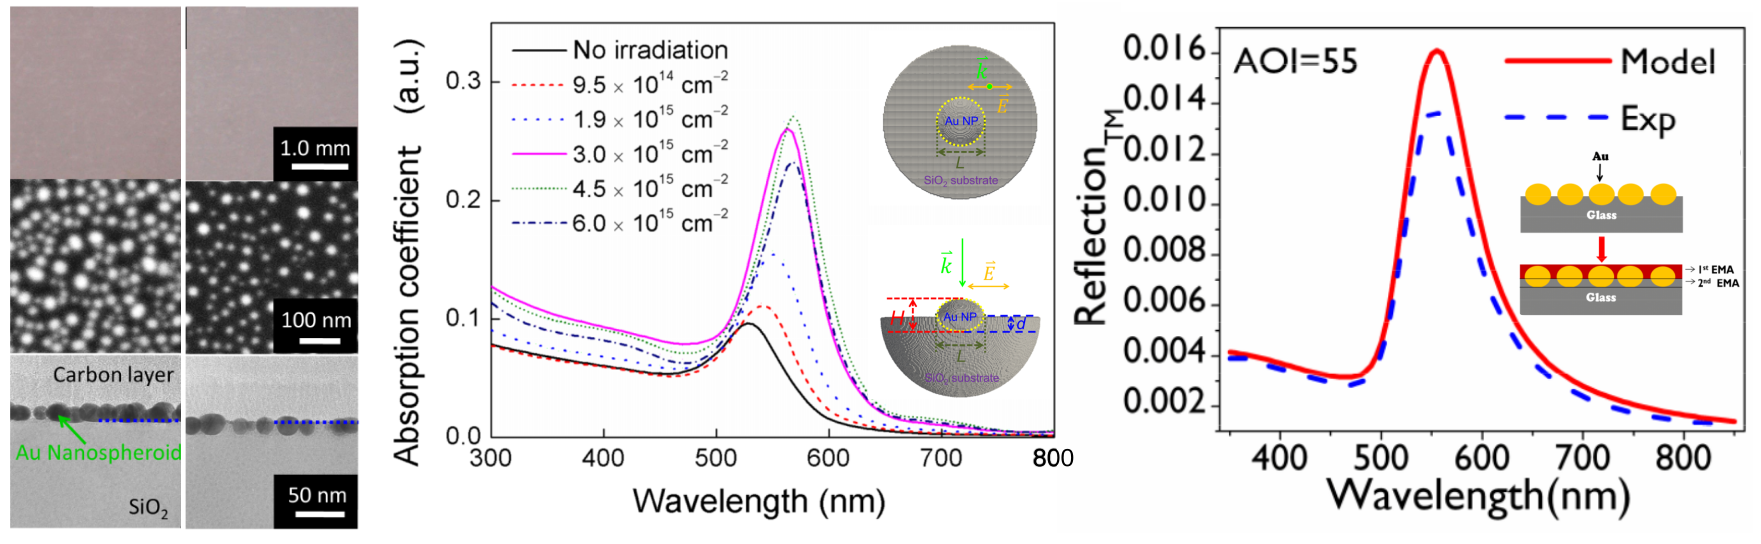
\includegraphics[width = .9\textwidth]{embedding.png}};
		\node at (-7.5,2.15) {  \begin{subfigure}{.2\textwidth}\caption{ }\label{sfig:inc:a}\end{subfigure}};
		\node at (-3.5,2.15) {  \begin{subfigure}{.2\textwidth}\caption{ }\label{sfig:inc:b}\end{subfigure}};
		\node at (1.725,2.15) {  \begin{subfigure}{.2\textwidth}\caption{ }\label{sfig:inc:c}\end{subfigure}};
\end{tikzpicture}
  \vspace*{-.75em}
  \caption[Backgrounds]{Previous works on partially embedded Au nanospheroids. \textbf{a)} Optical image and Transmission Electron Microscopy (TEM) images in an aerial and transversal view of disordered bidimensional arrays of nanospheres supported on silica  (SiO$_2$),  with two different incrustation degrees, fabricated by laser ablation of a Au thin film; image extracted and adapted from \cite{meng_anisotropic_2015}. \textbf{b) }  Absorption coefficient of a single Au nanospheroid ---with a semi-major (semi-minor) axis of $L$ ($H$)--- when illuminated at normal incidence by a plane wave, calculated through DDA calculations considering the measured dimensions and incrustration degree of the Au nanospheres when illuminated at different fluences (see inset list); images extracted and adapted from \cite{meng_anisotropic_2015}.  \textbf{c)} Experimental and theoretical reflectivity, as a function of the wavelength, of a disordered bidimensional array of partially embedded Au nanospheres illuminated at an angle of incidence (AOI) of $55^\circ$ with a transverse magnetic (TM) polarization state; the employed model consisted on substituting the partially embedded Au nanospheres by two layers whose optical response is described by the Maxwell Garnet Model with fitting parameters; images extracted and adapted from \cite{moirangthem_enhanced_2012}.
   }
\label{fig:IncPapers}
\end{figure}

In this thesis, the optical properties of a single Au nanosphere partially embedded in a substrate are studied when illuminated by a monochromatic plane wave at an oblique incidence with a defined polarization state. The motivation for such a physical system arises from the collaboration between two experimental research groups\footnote{The Biophotonics Group and the Organic and Hybrid Semiconductor Optoelectronics Group at \textit{Instituto Nacional de Astronomía, Óptica y Electrónica} (INAOE).} and one theoretical research group\footnote{The Nanoplasmonics Group at \textit{Facultad de Ciencias, Universidad Nacional Autónoma de México} (UNAM).}. The experimental groups have fabricated disordered arrays of partially embeded Au nanospheres with an average radius of $12.5$ nm ---a potential meta-atom for biosensing-aimed metasurfaces---. Therefore, the system of interest in this thesis consists in a spherical Au nanoparticle of radius $12.5$ nm located at the planar interface between an air matrix and a glass substrate, whose embedding (including the perfectly supported and totally incrusted nanosphere) is characterized by the incrustation parameter: the height of the center of the nanosphere relative to the interface divided by its radius. To determine the optical response of the system, the scattering and absorption efficiencies, the radiation pattern and the spatial distribution of induced electric field of the partially embedded nanosphere are calculated by means of the FEM ---implemented in the commercial software COMSOL Multiphysics\texttrademark{} Ver. 5.4 (COMSOL)--- and they are compared with the results obtained with the Mie Theory ---the analytical solution of the limiting case of a single nanosphere embedded in a infinite medium---, which allows to estimate the performance of partially embedded nanoshperes in metasurfaces tailored for biosensing.

The structure of this thesis divides its contents in three main chapters as follows: the scatering theory of single spherical particles is presented in Chapter \ref{ch:OpticalProperties}, beginning with the general case of arbitrary particles in Section \ref{s:AmpMatCrossSect} and followed by the particular case of spherical scatterers,  giving rise to the development of the Mie Theory in Section \ref{s:Mie}, which includes the derivation of the Vector Spherical Harmonics (Section \ref{ss:VSH}) and the explicit solution to the scattered and internal electromagnetic fields (Section \ref{ss:Fields}); in Section \ref{ss:AuMie} the optical properties of a Au nanosphere of radius $12.5$ nm embedded in air, and in glass, are calculated as the Mie-limiting case to the system of interest. Chapter \ref{chapter:FEM} aims at providing the fundamentals of the FEM in Section \ref{s:FEM-Fund}, including the Galerkin Method in Section \ref{s:FEM-Fund} and the characteristics of the Finite Element Approximation to a problem of partial differential equations in Section \ref{ss:FEM-FE}, and how the light scattering problem is addressed in the FEM in Section \ref{s:Scat-FEM}, which yields its Strong and Weak formulations (Section \ref{ss:Scat-Form}), the kind of finite element suited for the light scattering problem ---the Nédélec Finite Element--- (Section  \ref{ss:Nedelec}), and the so-called Open Boundary Conditions (Section  \ref{ss:Sommerfeld-PML}) that allows to calculate optical properties for infinite non-periodic  systems, as that of a single partially embedded nanosphere; after the theory of the FEM is presented, a convergence analysis is presented in Section \ref{sec:FEM-Mie} for the FEM implementation in COMSOL where its results are compared against the analytical solutions calculated by the Mie Theory. Then, the obtained results and their discussion are presented in Chapter \ref{ch:Results}, which corresponds to the scattering and absorption efficiencies, the radiation patterns and the spatial distribution of the induced electric field of a Au nanosphere of radius $12.5$ nm under the following conditions: perfect support and total embedding in the substrate in Section \ref{s:Totally}, and partial embedding in Section \ref{s:Emb}; the first considers normal incidence illumination in both an internal and external illumination schema in Section \ref{s:Totally:Normal} and in a Total Internal Reflection Configuration (TIR) in Section \ref{s:TIR}, while the second addresses the normal illumination case only in internal illumination and the TIR configuration in Sections \ref{s:Emb:Normal} and \ref{s:Emb:Obl}, respectively. Lastly, the \hyperref[ch:Conclusions]{Conclusions} of this work and its \hyperref[s:FWork]{future application on Metasurfaces} are located after the three main chapters.	


As a complementary material, there are included three appendices describing the conventions employed for the calculations with the Mie Theory (Appendix \ref{app:MieCode}), the size correction to the dielectric function for small spherical nanoparticles (Appendix \ref{app:SizeCorrection}) ---both available in the public GitHub repository \href{https://github.com/jaurrutia/Mie-Theory-Mathematica}{jaurrutia/Mie-Theory-Mathematica}--- and a brief guide of how the performed calculations were implemented in COMSOL (Appendix \ref{app:COMSOL}).







%\part{Theoretical Framework}
\chapter{Scattering Theory of a Single Spherical Particle}
  \label{ch:OpticalProperties}

	\section{The Optical Theorem: Amplitude Matrix and Cross Sections}
	 \label{s:AmpMatCrossSect}
	 % !TeX root = ../tesis.tex

Let $\vb{E}^\text{i} = \vb{E}^\text{i}_0 \exp(i\vb{k}^\text{i}\cdot\vb{r})$ be the electric field of an incident monochromatic plane wave with constant amplitude $\vb{E}_0^\text{i}$  traveling through a non absorbing medium with refractive index $n_\text{mat}$, denominated as the matrix, in the direction $\vb{k}^\text{i} = k\vu{k}^\text{i}$, with $k = (\omega/c)n_\text{mat}$ the wave number of the plane wave in the matrix, and let $\vb{E}^\text{sca}$ be the scattered electric field due to a particle with arbitrary shape embedded in the matrix. In general, the scattered electric field propagates in all directions but for an observation point $\vb{r} = r\vu{e}_r$, the traveling direction is defined by the vector $\vb{k}^\text{sca} = k\vu{k}^\text{sca} = k\vu{e}_r$.  Due to the linearity of the Maxwell's equations,   the incident and scattered electric fields  in the far-field regime are related by the following linear relation \cite{tsang_scattering_2000}:
% --------------------------------- index entries ----------------------------------
\index{Plane!Wave}%
\index{Wave!Plane}%
% ------------------------------------------------------------------------------------
% ---------------------------------- eq: ScatAmpMat ----------------------------------
 \begin{equation}
	\vb{E}^\text{sca} =   \frac{\exp(i\vb{k}^\text{sca}\cdot\vb{r})}{r} \mathbb{F}(\vu{k}^\text{sca}, \vu{k}^\text{i}) \vb{E}^\text{i},
 \label{eq:ScatAmpMat}
 \end{equation}
% ---------------------------------- eq: ScatAmpMat ----------------------------------
%
where $\mathbb{F}(\vu{k}^\text{sca}, \vu{k}^\text{i})$ is the scattering  amplitude matrix from direction $\vu{k}^\text{i}$ into $\vu{k}^\text{sca}$. Since only the far-field is considered, both the incident and the scattered electric fields can be decomposed into two linearly independent components perpendicular to $\vb{k}^\text{i}$ and $\vb{k}^\text{sca}$, respectively, each forming a right-handed orthonormal system. If the particle acting as a scatterer has a symmetric shape, it is convenient to define an orthonormal system relative to the scattering plane, which is the plane containing $\vb{k}^\text{i}$ and $\vb{k}^\text{sca}$, since the elements of $\mathbb{F}(\vu{k}^\text{sca}, \vu{k}^\text{i})$ are simplified when represented in these bases \cite{tsang_scattering_2000}. In Fig. \ref{fig:ScatPlane} a plane wave traveling in the $z$ direction illuminates an arbitrary particle centered at the origin of the coordinate system and the scattering plane is depicted in green. By defining the directions perpendicular  ($\perp$) and parallel ($\parallel$) to the scattering plane,  the incident and scattered electric fields can be written as
% --------------------------------- index entries ----------------------------------
\index{Scattering!Amplitude Matrix@{Amplitude Matrix $\mathbb{F}$}}%
\index{Scattering!Plane!Unit Vector System}%
\index{Plane!Scattering!Coordinate System}%
\index{Scattering!Plane!Coordinate System}%
 \index{Coordinate System!Relative to Scattering Plane}%
% ------------------------------------------------------------------------------------
% ---------------------------------- eq:Ei // eq:Es ------------------------------
 \begin{align}
	\vb{E}^\text{i} & =  \qty(E_\parallel^\text{i}\vu{e}^\text{i}_\parallel + E_\perp^\text{i} \vu{e}_\perp^\text{i}) \exp(i\vb{k}^\text{i}\cdot\vb{r}),
 \label{eq:Ei} \\
	\vb{E}^\text{sca} & = \qty(E_\parallel^\text{sca}\vu{e}^\text{sca}_\parallel + E_\perp^\text{sca} \vu{e}_\perp^\text{sca}) \frac{\exp(i\vb{k}^\text{sca}\cdot\vb{r})}{r},
 \label{eq:Es}
 \end{align}
% ---------------------------------- eq:Ei // eq:Es ------------------------------
%
where a harmonic time dependence $\exp(-i\omega t)$ has been omitted, and it has been assumed that the scattered field is described by a spherical wave; the superscript `$\text{i}$' (`$\text{sca}$') denotes the orthonormal system defined by the incident plane wave (scattered fields).  Since $\{\vu{e}_\perp^\text{i}, \vu{e}_\parallel^\text{i},\vu{k}^\text{i} \}$ and $\{\vu{e}_\perp^\text{sca}, \vu{e}_\parallel^\text{sca},\vu{k}^\text{sca} \}$ ---shown in purple in Fig. \ref{fig:ScatPlane}  along with the Cartesian (blue) and spherical (black) unit vector bases--- are right-handed orthonormal systems, they are related as follows
%
% ---------------------------------- eq:eParaPerpPerp ------------------------------
 \begin{align}
	\vu{e}_\perp^\text{i} = \vu{e}_\perp^\text{sca}  & =  \vu{k}^\text{sca} \times \vu{k}^\text{i},
		\qquad
	\vu{e}^\text{i}_\parallel = \vu{k}^\text{i}\times \vu{e}^\text{i}_\perp,
		\qquad\text{and}\qquad
	\vu{e}^\text{sca}_\parallel = \vu{k}^\text{sca} \times \vu{e}_\perp^\text{sca}.
 \label{eq:eParaPerp}
 \end{align}
% ---------------------------------- eq:eParaPerpPerp ------------------------------
%
% -------------------------------------- Scattering plane vector system  -------------------------------
% -------------------------------------- Scattering plane vector system  -------------------------------
% --------------------------------------          fig:ScatPlane          -------------------------------
\begin{figure}[!bht]\centering
	\tdplotsetmaincoords{60}{110}
 \pgfmathsetmacro{\rvec}{1. 3}
 \pgfmathsetmacro{\thetavec}{30}
 \pgfmathsetmacro{\varphivec}{60}
\begin{tikzpicture}[scale=3.5,tdplot_main_coords]
 %draw the NP
 %\draw[tdplot_screen_coords,ball color=yellow, opacity = 1] (0,0,0) circle (.05);
 %\draw[tdplot_screen_coords, color=yellow, opacity = 1] (0,0,0) circle (.05);

 \pgfmathsetseed{3}
     \draw[tdplot_screen_coords, ball color=yellow, opacity = 1,scale =.075]
     plot [smooth cycle, samples=8,domain={1:8}]
         (\x*360/8+5*rnd:0.5cm+1cm*rnd) node at (0,0) {};
 \pgfmathsetseed{3}
     \draw[tdplot_screen_coords, color=yellow, opacity = 1,scale =.075]
      plot [smooth cycle, samples=8,domain={1:8}]
      (\x*360/8+5*rnd:0.5cm+1cm*rnd) node at (0,0) {};


 % Set up some coordinates
  \coordinate (O) at (0,0,0);

 %determine a coordinate (P) using (r,\theta,\varphi) coordinates.   This command
 %also determines (Pxy), (Pxz), and (Pyz): the xy-, xz-, and yz-projections
 %of the point (P).
 %syntax: \tdplotsetcoord{Coordinate name without parentheses}{r}{\theta}{\varphi}
 \tdplotsetcoord{P}{\rvec}{\thetavec}{\varphivec}

 %draw figure contents
 %--------------------
 %draw the main coordinate system axes
     \draw[thick,- latex] (0,0,0) -- (1. 5,0,0) node[anchor=north east]{$x$};
     \draw[thick,- latex] (0,0,0) -- (0,1. 5,0) node[anchor=north west]{$y$};
     \draw[thick,- latex] (0,0,0) -- (0,0,1. 5) node[anchor=south]{$z$};

 %draw the main cartesian vector system
     \draw[thick,- latex, blue] (0,0,0) -- (1,0,0) node[anchor= south east]{$\vu{e}_x$};
     \draw[thick,- latex, blue] (0,0,0) -- (0,1,0) node[anchor=north west]{$\vu{e}_y$};
     \draw[thick,- latex, blue] (0,0,0) -- (0,0,1) node[anchor= east]{$\vu{e}_z$};

 %draw a vector from origin to point (P)
     \draw[thick,color=green, - latex] (O) -- (P);
     \node at (1,. 5,1. 1) {\color{green} $\vb{r}$};

 %draw projection on xy plane, and a connecting line
     \draw[dashed, color=green] (O) -- (Pxy);
     \draw[dashed, color=green] (P) -- (Pxy);
     \fill[green, opacity = .3] (O) --(Pxy)-- (P)--(O);
     \draw[- latex, tdplot_screen_coords,green](.42,.2)--(.8,.2);
     \node[tdplot_screen_coords] at (1.2,.2) {\color{green}\small Scattering plane};


 %draw the angle \varphi, and label it
     %syntax: \tdplotdrawarc[coordinate frame, draw options]{center point}{r}{angle}{label options}{label}
     \tdplotdrawarc[- latex]{(O)}{0. 5}{0}{\varphivec}{anchor=south}{$\varphi$}


 %set the rotated coordinate system so the x'-y' plane lies within the
     %"theta plane" of the main coordinate system
     %syntax: \tdplotsetthetaplanecoords{\varphi}
     \tdplotsetthetaplanecoords{\varphivec}

 %draw theta arc and label, using rotated coordinate system
     \tdplotdrawarc[tdplot_rotated_coords, - latex]{(0,0,0)}{0. 45}{0}{\thetavec}{anchor=north}{$\theta$}

 %draw some dashed arcs, demonstrating direct arc drawing
     \draw[dashed,tdplot_rotated_coords] (\rvec,0,0) arc (0:90:\rvec);
     \draw[dashed] (\rvec,0,0) arc (0:90:\rvec);

 %set the rotated coordinate definition within display using a translation
 %coordinate and Euler angles in the "z(\alpha)y(\beta)z(\gamma)" euler rotation convention
 %syntax: \tdplotsetrotatedcoords{\alpha}{\beta}{\gamma}
     \tdplotsetrotatedcoords{\varphivec}{\thetavec}{0}

 %translate the rotated coordinate system
 %syntax: \tdplotsetrotatedcoordsorigin{point}
     \tdplotsetrotatedcoordsorigin{(P)}

 %use the tdplot_rotated_coords style to work in the rotated, translated coordinate frame
     \draw[thick,tdplot_rotated_coords,- latex, purple] (0,0,0) -- (. 3,0,0) node[anchor=north west]{{\color{black}$\vu{e}_\theta,$}$\vu{e}_{\parallel}^\text{sca}$};
     \draw[thick,tdplot_rotated_coords,- latex,black] (0,0,0) -- (0,. 3,0) node[anchor=west]{$\vu{e}_\varphi$};
     \draw[thick,tdplot_rotated_coords,- latex,purple] (0,0,0) -- (0,-. 3,0) node[anchor= north west]{$\vu{e}_{\perp}^\text{sca}$};
     \draw[thick,tdplot_rotated_coords,- latex] (0,0,0) -- (0,0,. 3) node[anchor=south]{$\vu{k}^\text{sca}, \vu{e}_r$ };

 %set the rotated coordinate definition within display using a translation
 %coordinate and Euler angles in the "z(\alpha)y(\beta)z(\gamma)" euler rotation convention
 %syntax: \tdplotsetrotatedcoords{\alpha}{\beta}{\gamma}
     \tdplotsetrotatedcoords{\varphivec}{0}{0}

 %translate the rotated coordinate system
 %syntax: \tdplotsetrotatedcoordsorigin{point}
     \tdplotsetrotatedcoordsorigin{(Pxy)}

     \draw[thick,tdplot_rotated_coords,- latex, purple] (0,0,0) -- (. 3,0,0) node[anchor= west]{$\vu{e}_{\parallel}^\text{i}$};
     \draw[thick,tdplot_rotated_coords,- latex, blue] (0,0,0) -- (0,0,. 3) node[anchor= west]{$\vu{e}_z$};
     \draw[thick,tdplot_rotated_coords,- latex, purple] (0,0,0) -- (0,-. 3,0) node[anchor= north west]{$\vu{e}_{\perp}^\text{i}$};

 % plane wave
     \foreach \i in {-5}{%{-7,...,-2}{
         \draw[thick,tdplot_screen_coords,red, - latex] (\i/10,0,0)--(\i/10,1,0);}
     \node[tdplot_screen_coords] at (-4.75/10,1.1,0){\color{red}$\vb{k}^\text{i}$};
     \node[tdplot_screen_coords] at (-4.5/10,-.15,0){\begin{minipage}{2.cm}\centering\small \color{red}Incident plane wave\end{minipage}};
\end{tikzpicture}%

    \caption[Scattering plane unit vector systems]{The scattering plane (green) is defined by the vector $\vu{k}^\text{i}$ (red) parallel to $\vu{e}_z$ ---the direction of the incident plane wave--- and the vector $\vu{k}^\text{sca}$ ---the direction of the scattered field in a given point $\vec{r}$---. The parallel and perpendicular components of the incident field relative to the scattering plane are $\vu{e}_\parallel^\text{i} = \cos\varphi\,\vu{e}_x +\sin\varphi\,\vu{e}_y$ and  $\vu{e}_\perp^\text{i} = -\vu{e}_\varphi$, while the components of the scattering field relative to the scattering plane are $\vu{e}_\parallel^\text{sca} = \vu{e}_\theta$, $\vu{e}_\perp^\text{sca} = - \vu{e}_\varphi$. The Cartesian unit vector basis is shown in blue, the spherical unit vector basis in black, while the basis of the orthonormal systems relative to the scattering plane are shown in purple. }
    \label{fig:ScatPlane}
\end{figure}
% --------------------------------------          fig:ScatPlane          -------------------------------
%
\noindent
As Eqs. \eqref{eq:eParaPerp} suggest, the unit vector bases of the orthonormal systems relative to the scattering plane depend on the scattering direction. For example, if the incident plane wave travels along the $z$ axis (Fig. \ref{fig:ScatPlane}), then $\vu{k}^\text{i} = \vu{e}_z$ and $\vu{k}^\text{sca} = \vu{e}_r$. Thus the unit vector bases of the systems relative to the scattering plane are   $\vu{e}_\parallel^\text{i} = \cos\varphi\, \vu{e}_x +\sin\varphi\, \vu{e}_y$, $\vu{e}_\parallel^\text{sca} = \vu{e}_\theta$ and $\vu{e}_\perp^\text{i} = \vu{e}_\perp^\text{sca}  = - \vu{e}_\varphi$, with $\theta$ the polar angle and $\varphi$ the azimuthal angle.

When an incident plane wave interacts with a particle with a complex refractive index $n_\text{p}(\omega)$, the total electric field outside the particle is given by the sum of the incident and the scattered fields. Therefore, the time averaged Poynting vector $\ev{\vb{S}}_t$, denoting the power flow per unit area, of the total field is given by
% --------------------- index entries----------------------
\index{Vector!Time Averaged Poynting@{Averaged Poynting $\ev{\vb{S}}_t$}}%
% ------------------------------------  eq:Stot   ---------------------
\begin{align}
	\ev{\vb{S}}_t
		= \underbrace{\frac12 \Re \qty(\vb{E}^\text{i}\times\vb{H}^\text{i*})}_{\text{\normalsize $\ev{\vb{S}^\text{i}}_t $}} +
		  \underbrace{\frac12 \Re \qty(\vb{E}^\text{sca}\times\vb{H}^\text{sca*})}_{\text{\normalsize $\ev{\vb{S}^\text{sca}}_t $}}+
		   \underbrace{	\frac12 \Re\qty(\vb{E}^\text{i}\times\vb{H}^\text{sca*} + \vb{E}^\text{sca}\times\vb{H}^\text{i*})}_{\text{\normalsize$\ev{\vb{S}^\text{ext}}_t$}},
 \label{eq:Stot}
\end{align}
% ------------------------------------  eq:Stot   ---------------------
%
with $^*$  the complex conjugate operation and where the total Poynting vector is separated in three terms: the contribution from the incident field $\ev{\vb{S}^\text{i}}_t$, from the scattered field $\ev{\vb{S}^\text{sca}}_t$ and from their cross product denoted by $\ev{\vb{S}^\text{ext}}_t$. By means of the Faraday-Lenz's law and Eqs. \eqref{eq:ScatAmpMat}--\eqref{eq:Es}, the  contribution to the Poynting vector from the incident and the scattered fields can be rewritten as
% --------------------- index entries------------------------------------
\index{Faraday-Lenz's!Law}%
\index{Law!Faraday-Lenz's}
% ------------------ eq:AvePoyntingISca ---------------------------------
\begin{equation}
	\ev{\vb{S}^\text{i}}_t = \frac{\norm{\vb{E}_0^\text{i}}^2}{2 Z_\text{mat}}\vu{k}^\text{i},
		\qquad\text{and}\qquad
	\ev{\vb{S}^\text{sca}}_t = \frac{\norm{\vb{E}^\text{sca}}^2}{2 Z_\text{mat}}\vu{k}^\text{sca}
						=  \frac{\norm{\mathbb{F}(\vu{k}^\text{sca},\vu{k}^\text{i})\vb{E}^\text{i}}^2}{2 Z_\text{mat}r^2}\vu{k}^\text{sca},
 \label{eq:AvePoyntingISca}
\end{equation}
% ------------------ eq:AvePoyntingISca ---------------------------------
%
with $Z_\text{mat} = \sqrt{\mu_\text{mat}/\varepsilon_\text{mat}}$ the impedance of the non-absorbing matrix, while the crossed contribution is given by
%
% ------------------ eq:AvePoyntingExt ----------------------------------
 \begin{align}
 \ev{\vb{S}^\text{ext}}_t = &\Re\left\{
								\frac{\exp[-i(\vb{k}^\text{sca}-\vb{k}^\text{i})\cdot\vb{r}]}{2 Z_\text{mat}r^2}
								\qty[\vu{k}^\text{sca}\qty(\vb{E}_0^\text{i}\cdot \mathbb{F}^*\vb{E}^\text{i*})
									-\mathbb{F}^*\vb{E}^\text{i*}	\qty(\vb{E}^\text{i}_0\cdot\vu{k}^\text{sca})]
							 \right.\notag	\\
							&\hspace{2em}\left.
								+\frac{\exp[i(\vb{k}^\text{sca}-\vb{k}^\text{i})\cdot\vb{r}]}{2 Z_\text{mat}r^2}
								\qty[\vu{k}^\text{i}\qty(\mathbb{F}\vb{E}^\text{i}\cdot\vb{E}^\text{i*}_0)
									-\vb{E}^\text{i*}_0 \qty(\mathbb{F}\vb{E}^\text{i}\cdot\vu{k}^\text{i})]	\right\},
 \label{eq:AvePoyntingExt}
\end{align}%
% ------------------ eq:AvePoyntingExt ----------------------------------%
where the scattering amplitude matrix is evaluated as $\mathbb{F}(\vu{k}^\text{sca},\vu{k}^\text{i})$.

The power scattered by the particle can be calculated by integrating $\ev{\vb{S}^\text{sca}}_t$ in a closed surface surrounding the particle; if the scattered power is normalized by the irradiance of the incident field $\norm{\ev{\vb{S}^\text{i}}_t}$, it is obtained a quantity with units of area, known as the scattering cross section $C_\text{sca}$, given by \cite{bohren_absorption_1983}%
% -------------------- index entries ------------------------------
\index{Plane!Wave!Irradiance}%
\index{Cross Section!Scattering@{Scattering $C_\text{sca}$}}%
\index{Scattering!Cross Section}%
% ------------------- eq:Csca --------------------------------------
 \begin{tcolorbox}[title = Scattering Cross Section,	ams align, breakable]
	C_\text{sca} = \frac{2Z_\text{mat}}{\norm{\vb{E}_0}^2} \oint_\mathcal{S} \ev{\vb{S}^\text{sca}}_t \cdot\dd{\vb{a}}
				= \oint_\mathcal{S} \frac{\norm{\mathbb{F}(\vu{k}^\text{sca},\vu{k}^\text{i})\vb{E}^\text{i}}^2}
									{\norm{\vb{E}^\text{i}_0}^2}\dd{\Omega},
 \label{eq:Csca}
 \end{tcolorbox}
% ------------------- eq:Csca --------------------------------------
%
\noindent
where $\dd{\Omega}$ is the differential solid angle.

Similarly, an absorption cross section $C_\text{abs}$ can be defined as well. On the one side, the absorption cross section is given by the integral on a closed surface of $\ev{-\vb{S}}_t$  [Eq. \eqref{eq:Stot}] divided by the irradiance of the incident field, where the minus sign is chosen so that $C_\text{abs}>0$ if the particle absorbs energy  \cite{bohren_absorption_1983}. On the other side, if an Ohmic material with conductivity $\sigma(\omega) = i\omega n_\text{p}^2(\omega)$ \cite{jackson_classical_1999} for the particle is assumed, through Joule's heating law \cite{tsang_scattering_2000}, the absorption cross section can be computed as
% ------------------------------------index entries ----------------
\index{Joule!Heating Law}%
\index{Ohm!Law}%
\index{Law!Joule Heating}%
\index{Law!Ohm}%
\index{Cross Section!Absorption@{Scattering $C_\text{abs}$}}%
\index{Absorption!Cross Section}%
% ------------------- eq:Cabs --------------------------------------
 \begin{tcolorbox}[title = Ohmic Particle - Absorption Cross Section,	ams align, breakable]
 	C_\text{abs} =	 \frac12\int_\mathcal{V} \frac{\Re(\vb{J}\cdot \vb{E}^\text{int*})}
 									{\norm{\vb{E}_0^\text{i}}^2/2Z_\text{mat}}\dd{V}
				= \int_\mathcal{V} \omega Z_\text{mat}\Im(n_\text{p}^2) \frac{\norm{\vb{E}^\text{int}}^2}{\norm{\vb{E}^\text{i}_0}^2} \dd{V},
 \label{eq:Cabs}
 \end{tcolorbox}%
% ------------------- eq:Cabs --------------------------------------
%
\noindent
where the integration is performed inside the particle, and $\vb{J}$  and $\vb{E}^\text{int}$ are the volumetric electric current density and the total electric field in this region, respectively. Both the  scattering and the absorption cross sections are quantities related to the optical signature of a particle \cite{pellarin_forward_2019}, and their relation can be made explicit by performing the surface integral representation of $C_\text{abs}$ and defining $C_\text{ext}$, that is,
%
% ------------------- eq:CabsScaInt ----------
\begin{align}
C_\text{abs} = & - \frac{2Z_\text{mat}}{\norm{\vb{E}^\text{i}_0}^2}\int_\mathcal{S}
                        \Big(
                                \ev{\vb{S}^\text{i}}_t + \Bigl\langle\vb{S}^\text{sca}\Bigr\rangle_t + \ev{\vb{S}^\text{ext}}_t
                        \Big)\cdot\dd{\vb{a}}
					\notag \\
			=  & - C_\text{sca} - \frac{2Z_\text{mat}}{\norm{\vb{E}_0^\text{i}}^2}\int_\mathcal{S}
                        \ev{\vb{S}^\text{ext}}_t\cdot \vu{e}_r\dd{\Omega}
					\notag \\
			= & -C_\text{sca} + C_\text{ext},
\label{eq:CabsScaInt}
\end{align}
% -------------------- eq:CabsScaInt ----------
%
where the contribution of $\ev{\vb{S}^\text{i}}_t$ to the integral is zero since a non-absorbing matrix was assumed. From Eq. \eqref{eq:CabsScaInt} it can be seen that $C_\text{ext}$ takes into account both mechanisms for energy losses (scattering and absorption), thus it is called the extinction cross section. To solve the integral in Eq. \eqref{eq:CabsScaInt} let us define $\theta$ as the angle between $\vu{k}^\text{sca}$ and $\vu{k}^\text{i}$ as the polar angle  and  $\varphi$ as the azimuthal angle, as shown in Fig \ref{fig:ScatPlane}. With this choice of coordinates,  the extinction cross section can be computed as
% --------------------------- index entries ------
\index{Extinction!Cross Section}%
\index{Cross Section!Extinction}%
% ----------------------------- eq:CextFull ------
\begin{align}
C_\text{ext} = - &\Re \left\{
			 \frac{\exp(-ikr) }{\norm{\vb{E}_0^\text{i}}^2}
			 			\oint_\mathcal{S} \exp(ikr\cos\theta)\qty(\vb{E}^\text{i}\cdot \mathbb{F}^*\vb{E}^\text{i*})  \dd{\Omega} \right.	\notag\\
			&\hspace*{1.5em}+\frac{\exp(ikr) }{\norm{\vb{E}_0^\text{i}}^2}
						\oint_\mathcal{S} \exp(-ikr\cos\theta)\cos\theta \qty(\vb{E}^\text{i*}\cdot \mathbb{F}\vb{E}^\text{i})     \dd{\Omega}
\label{eq:CextFull}\\
			&\hspace*{1.5em}+\left.\frac{\exp(ikr) }{\norm{\vb{E}^\text{i}_0}^2}
						\oint_\mathcal{S} \exp(-ikr\cos\theta)\sin\theta(E_{0,x}^\text{i}\cos\varphi+E_{0,y}^\text{i}\sin\varphi)
									\qty(\mathbb{F}\vb{E}^\text{i}\cdot\vb{k}^\text{i})    \dd{\Omega}  \right\}, \notag
\end{align}
% ------------------------------ eq:CextFull -------
%
using that $\vu{k}^\text{sca}\cdot\vu{e}_r = 1$, $\vu{k}^\text{i}\cdot\vu{e}_r = \cos\theta$ and  $\vb{E}^\text{sca}\cdot\vu{e}_r = 0$. The integrals in Eq. \eqref{eq:CextFull} can be solved by a twofold integration by parts in the polar angle $\theta$ and by neglecting terms proportional to $r^{-2}$. This process leads to a zero contribution from the integrand proportional to $\sin\theta$  in Eq. \eqref{eq:CextFull} and, after rearranging the other terms in their real and imaginary parts, it follows that $C_\text{ext}$ depends only on the forward direction  $\vu{k}^\text{sca} = \vu{k}^\text{i}$ ($\theta =0$). This result is known as the Optical Theorem  whose mathematical expression is given by \cite{tsang_scattering_2000,pellarin_forward_2019,newton_optical_1976}:
% ------------------------index entries----
\index{Optical!Theorem}%
\index{Theorem!Optical}%
% --------------------------eq:Cext  ---
\begin{tcolorbox}[title = Optical Theorem - Extinction Cross Section,	ams align, breakable]
		C_\text{ext} = C_\text{abs} + C_\text{sca}
					=  \frac{4\pi}{k \norm{\vb{E}_0^\text{i}}^2}&\Im\qty[ \vb{E}_0^\text{i}\cdot \mathbb{F}^*(\vu{k}^\text{i},\vu{k}^\text{i}) \vb{E}^\text{i*} ].
\label{eq:Cext}
\end{tcolorbox}
% ------------------------ eq:Cext ------
%
\noindent The Optical Theorem is a general result applicable to general scattering phenomena, both quantum and classical  \cite{bohren_absorption_1983,newton_optical_1976}, and its derivation rely in the incident field being a plane wave [see Eq. \eqref{eq:CextFull}] and more precisely, in the lack of longitudinal components of the incident field \cite{krasavin_generalization_2018,born_max_principle_1999}.

From Eqs. \eqref{eq:Stot} and  \eqref{eq:Cext} it can be seen that the extinction of light, the combined result of scattering and absorption as energy loss mechanisms, is also a manifestation of the interference between the incident and the scattered fields and, remarkably,  that the overall effect of the light extinction can be fully understood by analyzing the  amplitude of the scattering field in the forward direction.  It is worth noting that Eq. \eqref{eq:Cext} is an exact relation but its usefulness is bond to the correct evaluation of the scattering amplitude matrix $\mathbb{F}$ \cite{tsang_scattering_2000}. Thus, in the following Sections a scattering problem with spherical symmetry will be assumed, so that the exact solution to the scattering amplitude matrix can be developed; this solution is known as the \emph{Mie Theory}.



%     In the previous Section, it was concluded that the extinction of light due to the interaction between a particle and a monochromatic plane wave can be determined through the amplitude of the scattered field in the forward direction. This is stated in the Optical Theorem, which is an exact relation, but inaccuracies may arise when either the scattering amplitude matrix or the extinction cross section are approximated\footnote{See for example Section 2.4 from Ref. \cite{tsang_scattering_2000} on the Rayleigh Scattering, and Section 21.7 from Ref. \cite{zangwill_modern_2013} on Thompson scattering.}. A particular case in which the scattering amplitude matrix can be exactly calculated is when the scatterer has spherical symmetry. In order to address this special case, it will be introduced a vectorial basis with spherical symmetry, known as the Vector Spherical Harmonics (VSH). Once the VSH are defined, they will be used to write a monochromatic plane wave in terms of the VSH. By imposing the continuity of the tangential components of the electric and magnetic fields, the scattered field can be also written in terms of the VSH. As a particular example of interest, shown in the last Section, the optical properties of a gold nanoparticle with radius of $12.5$ nm are calculated.
%
%     % ------------------------------- index entries --------
%     \index{Scattering!Thompson}%
%     \index{Scattering!Mie}%
%     \index{Scattering!Rayleigh}%
%     \index{Vector!Spherical Harmonics}%

\chapter{Results and Discussion}
	\label{ch:Results}

    \section{Supported and Totally Embedded Spherical Particles}
     \label{s:Totally}
        % !TeX root = ../tesis.tex

To compare the optical response of a NP in the presence of a substrate with that of a NP in a totally homogeneous environment, let us first analyze the spectral response given by the Mie Theory when the matrix and the size of the NP varies. In Fig. \ref{fig:Mie:redshift} it is shown the wavelength of resonance $\lambda_\text{res}$, that is, the wavelength at which the scattering (orange) and extinction (black) efficiencies are maximized,  as a  function of the radius $a$ of a AuNP embedded in a matrix of air [Fig. \ref{sfig:red:1}] and of glass [Fig. \ref{sfig:red:2}], with a refractive index of $n_\text{m} = 1$ and $n_\text{m} = 1.5$, respectively, and as a function of the refractive index of the matrix $n_\text{m}$ for a AuNP with a radius of {$a = 12.5$ nm} [Fig. \ref{sfig:red:3}] and with a radius of $a = 50$ nm [Fig. \ref{sfig:red:4}]. For the optical response of the AuNP it was employed the experimental data as reported by \citeauthor{johnson_optical_1972} \cite{johnson_optical_1972} (filled circles) and by considering a size correction ---see Appendix \ref{app:SizeCorrection}--- to it (empty circles).

\begin{figure}[h!]
    \def\svgwidth{\textwidth}
    \includeinkscape[pretex = \small]{Redshift/redshift}
    \vspace*{-20.9em} \\
    \hspace*{1em}%
        \begin{subfigure}{.225\textwidth}\caption{AuNP$@$Air}\label{sfig:red:1}\end{subfigure}%
        \begin{subfigure}{.28\textwidth}\caption{AuNP$@$Glass}\label{sfig:red:2}\end{subfigure}%
        \begin{subfigure}{.225\textwidth}\caption{12.5 nm AuNP}\label{sfig:red:3}\end{subfigure}%
        \begin{subfigure}{.24\textwidth}\caption{50 nm AuNP}\label{sfig:red:4}\end{subfigure}
    \vspace*{16.5em}\\
    \caption[Spectral redshift of the scattering and extinction  efficiencies of a spherical AuNP as a function of its size and the embedding media]{Resonance wavelength $\lambda_\text{res}$ of the scattering (orange) and extinction (black) efficiencies of a AuNP as a function of the NP's radius when embedded \textbf{a)} in air ($n_\text{m} = 1)$ and \textbf{b)} in glass ($n_\text{m} = 1.5$), and as a function of the refractive index of the matrix  $n_\text{m}$ for a AuNP of radius \textbf{c)} 12.5 nm and \textbf{d)} 50 nm, using the dielectric function for gold as reported by \citeauthor{johnson_optical_1972} \cite{johnson_optical_1972} (filled circles) and considering a size correction to it (empty circles).}
    \label{fig:Mie:redshift}
\end{figure}

From the results shown in Fig. \ref{fig:Mie:redshift} it can be seen that the wavelength of resonance  $\lambda_\text{res}$ for the extinction, considering the bulk dielectric function for Au (filled circles), is smaller than that of the scattering  and that the distance between them decreases as either the size of the AuNP or the refractive index of the matrix increases. This behavior arises from a redshift of $\lambda_\text{res}$ for increasing values of $a$ and $n_\text{m}$ and it shows that, for particles small compared to the wavelength of the incident light in the matrix, the main contribution to the extinction of light  is due to absorption processes and as the size of the AuNP grows, the extinction is dominated by its other contribution: the scattering, as discussed in Section \ref{ss:AuMie} and supported by Eq. \eqref{eq:Cext}. The redshift of   $\lambda_\text{res}$ can also be observed when considering a size corrected dielectric function (empty circles). Remarkably, for values of radius $\lesssim 15/n_\text{m}$ there is a blueshift of $\lambda_\text{res}$, as it can be seen in Figs. \ref{sfig:red:1} and \ref{sfig:red:2}, which is a consequence of a greater imaginary part of the dielectric function for the AuNP due to the size correction. On the other hand, an increase in $n_\text{m}$ for a fixed radius presents only redshifts either with or without a size corrected dielectric function [see Figs. \ref{sfig:red:3} and  \ref{sfig:red:4}].

The spectral behavior of the scattering and extinction of light due to a spherical NP summarized in Fig. \ref{fig:Mie:redshift} was calculated by assuming a homogeneous medium (the matrix) where the NP is embedded and thus allowing the direction of the illuminating plane wave to be arbitrary, yet yielding the same results. In the following Sections, the homogeneity of the surroundings of the NP is substituted by two semiinfinite media and thus modifying the optical response of the system depending on how it is illuminated.


        \subsection{Normal Incidence}
        % !TeX root = ../tesis.tex

The problem of scattering and absorption of light by single spherical NP embedded in a matrix, with refractive index $n_\text{m}$, illuminated by a plane wave with wavelength $\lambda$  and traveling in the  $\vb{k}^\text{i}$ direction, has spherical symmetry, which was exploited to develop the Mie Theory as explained in Section \ref{s:Mie}. If a substrate, with refractive index $n_\text{s}$, is considered and the NP is located right above or below the interface ---without crossing the substrate-matrix interface---, there are four combinations in which the system can be excited since the NP can be either embedded  in the substrate or supported on it, and it can be illuminated either in an external ---from the matrix to the substrate--- or in an internal ---from the substrate to matrix--- configuration, as shown in Fig. \ref{sfig:TotallyNormal:1}, where the following cases are depicted: Embedded-External (EE), Embedded-Internal (EI), Supported-External (SE) and Supported-Internal (SI). In the  presence of the substrate, the electric field illuminating the AuNP is not the incoming plane wave but the sum of it with the reflected electric field (EI and SE) or the transmitted electric field (EE and SI), both of which can be calculated analytically through Fresnel's reflection and transmission amplitude coefficients, as discussed in Appendix \ref{app:COMSOL}.

\begin{figure}[b!]
    \small
    \centering
    \hspace*{-.75\textwidth}%
        \begin{subfigure}{.4\textwidth}\caption{ }\label{sfig:TotallyNormal:1}\end{subfigure}%
        \begin{subfigure}{.25\textwidth}\caption{ }\label{sfig:TotallyNormal:2}\end{subfigure}\\[5em]
    \hspace*{-.35\textwidth}%
        \begin{subfigure}{.25\textwidth}\caption{ }\label{sfig:TotallyNormal:3}\end{subfigure}\\[-8.5em]
    \def\svgwidth{.95\textwidth}
    \includeinkscape{1-Totally/1-Efficiencies/1-Normal-Eff}%
    \vspace*{-.5em}
    \caption[Absorption and Scattering Efficiencies of a 12.5 nm AuNP above and below a planar Interface Illuminated at Normal Incidence]{\textbf{a)} Schematics of a AuNP embedded (E) in [supported (S) on] a glass substrate ($n_\text{s} = 1.5$) forming a planar interface with an air matrix ($n_\text{m} = 1$) and illuminated by a plane wave traveling normally to the air-glass interface in an external (E) and in an internal (I) configuration. \textbf{b)} Absorption $Q_\text{abs}$ and \textbf{c)} scattering $Q_\text{sca}$ efficiencies of a $12.5$ nm AuNP as a function of the wavelength $\lambda$ of the illuminating plane wave in different spatial configurations: EE (black), EI (orange), SE (blue) and SI (light orange). The green shaded region shows the two Mie-limiting cases of a  AuNP embedded in air and in glass; the magenta (AuNP and substrate) and cyan (Mie-limiting) markers correspond to the efficiencies evaluated at the wavelength of resonance for each case.
    }
\label{fig:TotallyNormal}
\end{figure}

In Figs. \ref{sfig:TotallyNormal:2} and \ref{sfig:TotallyNormal:3}  the absorption $Q_\text{abs}$ and scattering $Q_\text{sca}$ efficiencies are shown, respectively, as a  function of $\lambda$ for a AuNP of radius $a = 12.5$ nm in the Embedded-External (black), Embedded-Internal (orange), Supported-External (blue) and Supported-Internal (light orange) configurations; the green shaded regions correspond to the values between the two limiting cases given by the Mie theory: the AuNP embedded in air (lower boundary) and embedded in glass (upper boundary). The magenta markers correspond to the values of the efficiencies evaluated at the wavelength of resonance considering the presence of a substrate while the cyan markers correspond to the efficiencies at the resonance wavelength for the Mie-limiting cases.

From the results shown in Figs. \ref{sfig:TotallyNormal:2} and \ref{sfig:TotallyNormal:3}, it can be seen that both the absorption and scattering efficiencies of the four spatial configurations are of the same order of magnitud as the Mie-limiting cases and, even more, the values of the efficiencies for the embedded AuNP (black and orange lines) lie very close to the Mie-limiting case of the AuNP in glass (upper boundary of the green shaded region) and the same behavior is observed for the supported AuNP (blue and light orange lines) and the Mie-limiting case of a AuNP embedded in air (lower boundary of the green shaded region). The presence of a substrate yields an overall enhancement and damping of the scattering and the absorption efficiencies relative to the isolated NP, which depend on the illumination of the system since $Q_\text{abs}$ and $Q_\text{sca}$ are inversely proportional to the refractive index of the medium of incidence [Ecs. \eqref{eq:Csca} and \eqref{eq:Cabs}]: If the system is illuminated in an external configuration, the obtained efficiencies are slightly decreased relative to the Mie-limiting case as it can be seen from the black  and blue curves, which correspond to the EE and SE cases; on the other hand, the calculated efficiencies for the internal illuminated cases, that is for EI (orange) and SI (light orange), are enhanced relative to the Mie-limiting cases.

Another effect of the substrate in the optical response of the system is a slightly spectral shift of the excitation wavelength of the scattering and absorption efficiencies, which depends on the medium where the AuNP is located. For example, in Figs. \ref{sfig:TotallyNormal:2} and \ref{sfig:TotallyNormal:3} the wavelength of resonance for both the absorption and the scattering efficiencies (magenta markers)  are redshifted $\sim 1$ nm, relative to the Mie-limiting case (cyan markers), for the AuNP supported on the substrate (blue and light orange curves) and blueshifted $\sim 2$ nm for the embedded AuNP (black and orange curves). These spectral shifts can be understood by considering the AuNPs as electric point dipoles parallel to the interface ---an assumption consistent with the near-field distribution in the Mie-limiting cases and with the radiation patterns (see Figs.  \ref{fig:ScatteringMaps} and \ref{fig:NearField})--- and their interaction with the image electric point dipoles induced within the substrate \cite{meng_anisotropic_2015}. Both the dipoles induced in the AuNP and the image dipoles are parallel to the interface but its strength differs by  a factor of $A_\text{dip} = (\sqrt{n_j}-\sqrt{n_i}) / (\sqrt{n_j}+\sqrt{n_i})$ \cite{barrera1991optical}, where $n_{j}$ is the refractive index of the medium where the real dipole (the AuNP) is located and $n_i$ of the medium where the image dipole is induced. If the AuNP is embedded in the substrate, then $A_\text{dip}>0$ meaning that the induced dipole is parallel to the real dipole, which is a more energetic configuration that yields the spectral blueshift of the resonance. Conversely, if the AuNP is supported on the substrate then $A_\text{dip}<0$ and the induced dipole is antiparallel to the real dipole, leading to a less energetic configuration and to the redshift observed in Figs. \ref{sfig:TotallyNormal:2} and \ref{sfig:TotallyNormal:3}.%
\index{Dipole!Image!Strength}

The absorption and scattering efficiencies are integral quantities which describe the global behavior of the induced electric field $\vb{E}^\text{ind}$, which corresponds to the internal electric field $\vb{E}^\text{int}$ inside the AuNP and to the scattered electric field $\vb{E}^\text{sca}$ outside of it. The distribution of $\vb{E}^\text{ind}$, for a fixed wavelength, is studied in two spatial regimes: the far- and the near-field. To analyze the optical response in the first regime, the radiation patterns of the AuNP are obtained numerically by plotting the magnitude of the scattered electric field in the far-field regime\footnote{\label{fnote:Stratton:Chu}%
    The FEM returns the induced electric field by a scatterer in a neighborhood around it  and there is no guarantee that the returned electric field, even at the boundaries of the volume where the FEM simulation is performed, corresponds to the far-field regime.  To calculate the radiation pattern from the obtained induced electric field, COMSOL Multiphysics\texttrademark{} Ver. 5.4  employs the  Stratton-Chu formula \cite{comsol_wave}, which is a near-field to far-field  transformation that  propagates the known electric near-field  over a mathematical surface surrounding all the scatterers  to an arbitrary point \cite{anyutin_algorithm_2019}. The Stratton-Chu formula is obtained by employing the vectorial generalization of the Green's second identity with the electric and magnetic near-fields and the Green's function to the scalar Helmholtz equation multiplied by a normal vector to the integration surface \cite{stratton_diffraction_1939}.%
} %
 $\vb{E}^\text{sca}_\text{far}$ as a function of the angle relative to the normal direction to the interface. In Figs. \ref{fig:Far:Emb:Norm} and  \ref{fig:Far:Sup:Norm}, it is shown the radiation patterns of the embedded and the supported AuNP, respectively, for several values of the wavelength $\lambda$ of the incident plane wave, as well as considering an illumination of the system in an  [\textbf{a)} and \textbf{b})] external and in an  [\textbf{c)} and \textbf{d})] internal configuration; additionally, it is considered that the incident electric field is totally [\textbf{a)} and \textbf{c})] parallel to the scattering plane $\vb{E}^\text{i}_\parallel$ and [\textbf{b)} and \textbf{d})] perpendicular to the scattering plane $\vb{E}^\text{i}_\perp$.

\begin{figure}[b!]
    \centering
    \def\svgwidth{.8\textwidth}
    \hspace*{-.215\textwidth}%
    \vspace*{-.5em}%
        \begin{subfigure}{.32\textwidth}\caption{\footnotesize$\dfrac{\norm{\vb{E}^\text{sca}_\text{far}}}{\norm{\vb{E}^\text{i}}} \; [10^{-9}]$  }\label{sfig:Far:Emb:Norm:a}\end{subfigure}%
        \begin{subfigure}{.4\textwidth}\caption{\footnotesize$\dfrac{\norm{\vb{E}^\text{sca}_\text{far}}}{\norm{\vb{E}^\text{i}}} \; [10^{-9}]$  }\label{sfig:Far:Emb:Norm:b}\end{subfigure}\\
    \includeinkscape[pretex = \footnotesize]{1-Totally/4-5-Far-XY-Embedded/4-5-Far-XY-Embedded-External}\\
    %
    \def\svgwidth{.8\textwidth}
    \hspace*{-.215\textwidth}%
    \vspace*{-.5em}%
        \begin{subfigure}{.32\textwidth}\caption{\footnotesize$\dfrac{\norm{\vb{E}^\text{sca}_\text{far}}}{\norm{\vb{E}^\text{i}}} \; [10^{-9}]$  }\label{sfig:Far:Emb:Norm:c}\end{subfigure}%
        \begin{subfigure}{.4\textwidth}\caption{\footnotesize$\dfrac{\norm{\vb{E}^\text{sca}_\text{far}}}{\norm{\vb{E}^\text{i}}} \; [10^{-9}]$  }\label{sfig:Far:Emb:Norm:d}\end{subfigure}\\
    \includeinkscape[pretex = \footnotesize]{1-Totally/4-5-Far-XY-Embedded/4-5-Far-XY-Embedded-Internal}%
    \caption[ Radiation pattern of a AuNP totally embedded in a substrate illuminated at normal incidence ]{Radiation patterns of a AuNP (light yellow) of radius $a = 12.5$ nm, embedded in a substrate (light blue) and illuminated by an electric plane wave $\vb{E}^\text{i}$ with a wavelength $\lambda$, traveling in the $\vb{k}^\text{i}$ direction normal to the interface between the substrate ($n_\text{s} = 1.5$) and the matrix ($n_\text{m} = 1)$. The radiation patterns consider the illumination of the system  \textbf{a,b)} in an external and  \textbf{c,d)} in an internal configuration, and with an incident electric field \textbf{a,c)}  $\vb{E}^\text{i}_\parallel$ parallel to the scattering plane and \textbf{b,d)} $\vb{E}^\text{i}_\perp$ perpendicular to it.}
    \label{fig:Far:Emb:Norm}
\end{figure}

The radiation patterns of both the embedded  and the supported AuNP follow the same trend independently of the illuminating wavelength $\lambda$ but the amplitude is modulated by the scattering efficiencies shown in Fig. \ref{sfig:TotallyNormal:3}. For example, in the EE  and EI cases (Fig. \ref{fig:Far:Emb:Norm}) the scattered electric field (in the far-field) decreases its amplitude as the wavelength increases from $400$ nm to $480$ nm (black, orange and blue curves) and from   $550$ nm to $600$  nm, while it increases from $485$ nm to $542$ nm, near the wavelength of resonance for the scattering efficiency, see Fig. \ref{sfig:TotallyNormal:3}. Similarly, for the SE and SI cases the amplitude of the far-field is modulated by its scattering efficiency as it can be seen from comparing the radiation patterns in Fig. \ref{fig:Far:Sup:Norm} at $400$ mn (black), $480$ nm (blue) and  $527$ nm (purple), with the value of $Q_\text{sca}$ at those wavelengths  corresponding to a global maximum, a global minimum and a local maximum at the wavelength of resonance, respectively [see Fig. \ref{sfig:TotallyNormal:3}].

\begin{figure}[t!]
    \centering
    \def\svgwidth{.8\textwidth}
    \hspace*{-.215\textwidth}%
    \vspace*{-.5em}%
        \begin{subfigure}{.32\textwidth}\caption{\footnotesize$\dfrac{\norm{\vb{E}^\text{sca}_\text{far}}}{\norm{\vb{E}^\text{i}}} \; [10^{-9}]$  }\label{sfig:Far:Sup:Norm:a}\end{subfigure}%
        \begin{subfigure}{.4\textwidth}\caption{\footnotesize$\dfrac{\norm{\vb{E}^\text{sca}_\text{far}}}{\norm{\vb{E}^\text{i}}} \; [10^{-9}]$  }\label{sfig:Far:Sup:Norm:b}\end{subfigure}\\
    \includeinkscape[pretex = \footnotesize]{1-Totally/4-5-Far-XY-Supported/4-5-Far-XY-Supported-External}\\
    %
    \def\svgwidth{.8\textwidth}
    \hspace*{-.215\textwidth}%
    \vspace*{-.5em}%
        \begin{subfigure}{.32\textwidth}\caption{\footnotesize$\dfrac{\norm{\vb{E}^\text{sca}_\text{far}}}{\norm{\vb{E}^\text{i}}} \; [10^{-9}]$  }\label{sfig:Far:Sup:Norm:c}\end{subfigure}%
        \begin{subfigure}{.4\textwidth}\caption{\footnotesize$\dfrac{\norm{\vb{E}^\text{sca}_\text{far}}}{\norm{\vb{E}^\text{i}}} \; [10^{-9}]$  }\label{sfig:Far:Sup:Norm:d}\end{subfigure}\\
    \includeinkscape[pretex = \footnotesize]{1-Totally/4-5-Far-XY-Supported/4-5-Far-XY-Supported-Internal}%
    \caption[  Radiation pattern of a AuNP supported into a substrate illuminated at normal incidence ]{Radiation patterns of a AuNP (light yellow) of radius $a = 12.5$ nm, supported on a substrate (light blue) and illuminated by an electric plane wave $\vb{E}^\text{i}$ with a wavelength $\lambda$, traveling in the $\vb{k}^\text{i}$ direction normal to the interface between the substrate ($n_\text{s} = 1.5$) and the matrix ($n_\text{m} = 1)$. The radiation patterns consider the illumination of the system  \textbf{a,b)} in an external and  \textbf{c,d)} in an internal configuration, and with an incident electric field \textbf{a,c)}  $\vb{E}^\text{i}_\parallel$ parallel to the scattering plane and \textbf{b,d)} $\vb{E}^\text{i}_\perp$ perpendicular to it.}
    \label{fig:Far:Sup:Norm}
\end{figure}

The shape of the radiation pattern of a 12.5 nm AuNP in the presence of a substrate, either embedded or supported, resembles that of the isolated 12.5 AuNP discussed in Section \ref{sss:FarField} [see Fig. \ref{fig:ScatteringMaps}] in that it follows a two-lobe and a one-lobe pattern depending on the orientation of $\vb{E}^\text{i}$ relative to the scattering plane. If the incident electric field is parallel to the scattering plane, a two-lobe pattern aligned to the direction $\vb{k}^\text{i}$ of the incident ---and transmitted--- plane wave arises as it can be seen in the Figs. \ref{sfig:Far:Emb:Norm:a} and  \ref{sfig:Far:Emb:Norm:c} for the EE case, and Figs.  \ref{sfig:Far:Sup:Norm:a} and \ref{sfig:Far:Sup:Norm:c} for the EI scenario. Contrastingly, when the incident electric field is perpendicular to the scattering plane, the one-lobe pattern can be identified [see Figs. \ref{sfig:Far:Emb:Norm:b} and \ref{sfig:Far:Emb:Norm:d} (SE), and \ref{sfig:Far:Sup:Norm:b} and \ref{sfig:Far:Sup:Norm:d} (SI)]. By comparing the Mie-limiting radiation pattern (see Fig. \ref{fig:ScatteringMaps}) with the radiation patterns considering a substrate, the later loses the polar symmetry observed in the Mie-limiting case.  In particular, the amplitude of $\vb{E}^\text{sca}_\text{far}$ is larger when evaluated at the medium of incidence  than at medium of transmission; this asymmetry is observed for both illuminating configurations (external and internal) and it does not depend on whether the AuNP is supported or embedded. Rather, the spatial configuration of the system determines the overall value of the far-field: when the AuNP is embedded, the far-field amplitude is greater by a factor of $2.5$  than when the AuNP is supported ---see the axis scale in Figs. \ref{fig:Far:Emb:Norm} and \ref{fig:Far:Sup:Norm}---; this phenomenon  is a consequence of the two following physical mechanisms. The first one is the substrate having a greater refractive index than the matrix, thus making the optical response of the 12.5 nm AuNP as that of a larger NP ---but still small compared to the illuminating wavelength---, as in the Mie-limiting case. The second mechanism is the relative alignment of the electric point dipole induced within the AuNP ---small particle approximation to the AuNP--- and the induced electric dipole due to the interface, which is parallel when the AuNP is embedded into the substrate and antiparallel when supported on it, thus leading to a more energetic configuration when the AuNP is located inside the substrate than inside the matrix.

The radiation pattern, an optical property observed in the far-field regime, is a manifestation of the near-field spatial distribution ---see the footnote on page \pageref{fnote:Stratton:Chu}--- which can be calculated numerically through the FEM for a AuNP of radius $a = 12.5$ nm. The scattered electric field in the  far-field regime of a AuNP embedded or supported  [Figs. \ref{fig:Far:Emb:Norm} and \ref{fig:Far:Sup:Norm}] share some characteristics with the radiated field of an isolated AuNP (Mie-limiting case), and thus it should be for the near-field. In Fig. \ref{fig:Near:IntExt} it is shown the magnitude of the induced electric field $\vb{E}^\text{ind}$ when the AuNP is illuminated by a $y$-polarized incident electric field $\vb{E}^\text{i}$ traveling in the $\vb{k}^\text{i}$ direction, perpendicular to the interface between air and glass; the induced electric field is evaluated at the scattering plane $x = 0$, that is, the incident electric field has only a parallel contribution $\vb{E}^\text{i}_\parallel$ to the scattering plane. The wavelength $\lambda$ of the incoming plane wave is $\lambda =535.2$ nm for an embedded AuNP either illuminated externally [Fig.  \ref{sfig:Near:EE}] or internally  [Fig.  \ref{sfig:Near:EI}] and  $\lambda =510$ nm for a supported AuNP either illuminated externally [Fig.  \ref{sfig:Near:SE}] or internally  [Fig.  \ref{sfig:Near:SI}], which correspond to the wavelengths of the Localized Surface Plasmon Resonance (LSPR), that is, at the wavelength of maximum absorption.

\begin{figure}[t!]\centering
   \def\svgwidth{.75 \textwidth}
   \footnotesize
   \captionsetup[subfigure]{labelfont ={normal,bf,color = white}}
   \includeinkscape{1-Totally/2-NearY/2-NearY-EmbSup}\\[-32.6em]
   \hspace*{-.25\textwidth}
       \begin{subfigure}{.25\textwidth}\caption{ } \label{sfig:Near:EE}\end{subfigure}%
       \begin{subfigure}{.36\textwidth}\caption{ } \label{sfig:Near:EI}\end{subfigure}\\[13em]
   \hspace*{-.25\textwidth}
       \begin{subfigure}{.25\textwidth}\caption{ } \label{sfig:Near:SE}\end{subfigure}%
       \begin{subfigure}{.36\textwidth}\caption{ } \label{sfig:Near:SI}\end{subfigure}\\[15em]
   \caption[Induced Electric Field of a 12.5 nm Au Spherical NP embbeded into (supported on) a substrate illuminated at a normal incidence]{Magnitude of the electric field induced $\vb{E}^\text{ind}$ by a 12.5 nm AuNP   (dashed black lines) illuminated by an incident electric plane wave $\vb{E}^\text{i}$ traveling in the $\vb{k}^\text{i}$ direction perpendicular to the interface  (dashed white lines) between an air matrix ($n_\text{m} = 1$) and a glass substrate ($n_\text{s} = 1.5$) when the AuNP is  \textbf{a,b)} embedded in the glass substrate and \textbf{c,d)} supported on it; the system is illuminated \textbf{a,c)}  in an external and \textbf{b,d)} in an internal configuration at the resonance wavelength for the absorption efficiency.}
   \label{fig:Near:IntExt}
 \end{figure}

The spatial distribution of the near-field shown in Fig. \ref{fig:Near:IntExt} is consistent with the description and explanation of both the absorption and scattering efficiencies [Figs. \ref{sfig:TotallyNormal:2} and \ref{sfig:TotallyNormal:3}] and the radiation patterns of the embedded [Fig. \ref{fig:Far:Emb:Norm}] and the supported [Fig. \ref{fig:Far:Sup:Norm}] AuNP. The induced electric field is, in general, stronger when the AuNP is embedded in the substrate than when it is supported on it, as can be seen in the magnitude of the hotspots around the AuNP: reddish regions in Figs. \ref{sfig:Near:EE} and \ref{sfig:Near:EI} and bluish in Figs. \ref{sfig:Near:SE} and \ref{sfig:Near:SI}. These hotspots also verify that at the resonance wavelength, the main contribution to the electric fields is due to an electric dipolar moment since the characteristic two-lobe distribution of the near-field can be easily identified nevertheless, the lobes are not horizontally aligned to the AuNP's equator but farther from the substrate for the embedded AuNP and closer to it for the supported AuNP, as if the induced dipole ---in the small particle approximation, where the AuNP is treated as an electric point dipole--- is parallel (perpendicular) to the dipolar moment induced in the AuNP when it is embedded in (supported on) the substrate, as discussed above.

Throughout this Section, the optical properties of a 12.5 nm AuNP on the presence of a substrate considering four configurations were studied: the AuNP either embedded or supported and the system illuminated from under the substrate or from above. The choice of normal incidence to the system allowed the obtained results to be compared with the Mie-limiting case, which lead to the identification of similarities and differences among the four configurations. The differences in the optical response are associated to the broken symmetry due to the two semiinfinte media now considered \cite{meng_anisotropic_2015}, while the similarities arise since the system is always illuminated by a plane wave independently of the choice of the medium of incidence, yielding a mostly dipolar electric field. Therefore, in the next Section the oblique incidence case is addressed only when the AuNP is supported and illuminated in the internal configuration, since it is the only case with a different type illumination to the system: an evanescent wave for incidence angles above the critical angle $\theta_c =\arcsin(n_\text{m}/n_\text{s})$ \cite{born_max_principle_1999}.

         \label{s:Totally:Normal}
       

\chapter*{Conclusions}
\addcontentsline{toc}{chapter}{\protect\numberline{}Conclusions}
	\label{ch:Conclusions}
	% !TeX root = ../../protocolo.tex

In this thesis, the  optical properties of a spherical gold nanoparticle (AuNP) of radius $a = 12.5$~nm, partially embedded in an air matrix and in a glass substrate, was studied as a function of its embedding degree, characterized by the incrustation parameter $h/a$ ---with $h$ the position of the center of the AuNP relative to the planar air-glass interface---. By means of the Finite Element Method ---implemented in the commercial software COMSOL Multiphysics\texttrademark{} Ver. 5.4--- the absorption and scattering efficiencies, the radiation pattern and the spatial distribution of the induced electric field of the partially embedded 12.5~nm~AuNP were calculated when the AuNP was illuminated by an electromagnetic plane wave traveling at an oblique direction, with a defined polarization state; all numerical results were compared with the Mie-limiting cases calculated analytically, consisting in a 12.5~nm~AuNP embedded in an infinite matrix of air, and an infinite matrix of glass. From the preformed calculations, it was observed that the 12.5~nm~AuNP with partial embedding can be described by a mainly dipolar contribution, that its coupling with the incident light and the spatial distribution of the electric field enhancement on its surface can be tuned depending on the embedding of the AuNP and its illumination conditions, and that the optical response is maximized if the system is illuminated with an evanescent wave at an angle of incidence near the critical angle. More specifically, from the preformed  calculations the following can be concluded:

    \begin{itemize}
        \item \textbf{The optical response of a single partially embedded AuNP can be described by a mainly dipolar contribution.}\\
        The absorption and scattering efficiencies present only one global maximum in the visible spectrum, at which the spatial distribution of the electric field enhancement and its radiation pattern resemble that of an electric point dipole. This behavior can be extended to other materials of the matrix, the substrate and the nanosphere (of any size) as long as the scattering contribution to the extinction of light is small compared to the absorption contribution.
        %
        \item \textbf{There is a smooth transition between the two Mie-limiting cases as the nanosphere is partially embedded into the substrate.}\\
        The  wavelength of resonance of the absorption and scattering efficiencies of the partially embedded nanosphere is localized in between the two Mie-limiting cases, which consist in the nanosphere embedded in an infinite media (either the matrix or the substrate). Aditionally, the wavelength of resonance is redshifted from the resonance wavelength of the matrix Mie-limiting case to the resonance wavelength of the substrate Mie-limiting case, and this redshift is different for an $s$ or  for a $p$ polarized incident electric field.
        %
        \item \textbf{The optical response of the nanosphere resembles that of a supported (totally embedded) nanosphere if at most one eight of its volume is partially embedded in the substrate (matrix).}\\
        The supported and totally embedded nanosphere are the extreme cases of the partially embedded nanosphere when the sphere is tangential to the matrix-substrate interface. The absorption and scattering efficiencies of the partially embedded nanospheres, for both polarizations, are enhanced and redshifted in the same trend as the supported and totally embedded spheres as the angle of incidence of the incident light changes if at most one eight of the nanosphere crossed the interface.
        %
        \item \textbf{The optical properties of the partially embedded nanospheres are maximized if illuminated at an angle of incidence near the critical angle.}\\
        For any incrustation parameter and polarization state, the magnitude of the scattering and absorption efficiencies is enhanced ---for all wavelengths in the visble spectrum--- as the angle of incidence grows from zero to the critical angle, and they start to  diminish for angles of incidence above the critical angle. This behavior is due to the effect of an evanescent wave illuminating the system above the interface, whose penetration depth is maximum at the critical angle.
        %
        \item \textbf{The wavelength of resonance and the electric field spatial distribution of the partially embedded nanospheres for $s$ polarized illumination do not depend on the angle of incidence while they do for $p$ polarized illumination.}\\
        On the one hand, for $s$ polarization, the redshift of the resonance wavelength as the nanosphere is buried into the substrate, is  the same for all angles of incidence and the  electric field at the resonance wavelength is enhanced in two hotspots aligned parallel to the interface and on the surface of the nanosphere in the substrate side of the system. On the other hand, for $p$ polarization, the redshift of the resonance wavelength is different for each angle of incidence. For example, near the critical angle, the redshift is appreciable if more than half of the nanosphere is buried into the substrate, while for normal incidence the behavior is equivalent to the $s$ polarization case. On the spatial distribution, one hotspot is located in the matrix and other in the substrate, and their alignment is determined by the transmitted electric field; in particular, for angles above the critical angle, the hotspots are aligned perpendicular to the substrate.
    \end{itemize}

Finally, it can be concluded that the optical properties of a partially embedded spherical AuNP of radius 12.5 nm, with at most one eight of its volume buried into the substrate, is suited for interactions with elements in the matrix under internal illumination. If the system is illuminated with a $p$ polarized incident electromagnetic plane wave traveling at an angle  $\theta_i \gtrsim \theta_c$, the system is optimized to interact with its surroundings above the substrate since the optical response is maximized in the matrix. Therefore, partially embedded spherical AuNPs are strong candidates for meta-atoms conforming a disordered biosensing-aimed-metasurface.
	
	

\appendix

\chapter{Mie Theory (Conventions)}
  \label{app:MieCode}
  % !TeX root = ../tesis.tex

The Vector Spherical Harmonics (VSH) where defined in Section \ref{ss:VSH} in terms of their generating function $\psi(r,\theta,\varphi)$ which must satisfy the scalar Helmholtz equation [Eq.  \eqref{eq:HelmoltzScalar}]. By employing the separation of variables method,  it was determined that $\psi$ is the product of either $\sin(m\varphi)$ or $\cos(m\varphi)$, the associated Legendre functions $P_\ell^m(\cos\theta)$ and the spherical Bessel/Hankel functions $z_\ell(kr)$, which are solutions to Eqs. \eqref{eq:Phi}-\eqref{eq:Reqkr}. In this Section, it is discussed the chosen definitions for $P_\ell^m$, $z_\ell$ and related functions, as well as how to calculate them.

\section*{Radial Dependency: Spherical Bessel/Hankel Functions}

\index{Functions!Spherical Bessel@{Spherical Bessel $j_\ell(\rho)$ and $y_\ell(\rho)$}}%
\index{Functions!Spherical Hankel@{Spherical Hankel $h^{(1)}_\ell(\rho)$ and $h^{(2)}_\ell(\rho)$}}%
\index{Bessel!Spherical Functions@{Spherical Functions $j_\ell(\rho)$ and $y_\ell(\rho)$}}%
\index{Hankel!Spherical Functions@{Spherical Functions $h^{(1)}_\ell(\rho)$ and $h^{(2)}_\ell(\rho)$}}%
%
The radial dependency of the VSH is given by the two linearly independent solutions to Eq. \eqref{eq:Reqkr} which are the spherical Bessel function of first and second kind $j_\ell(\rho)$ and $y_\ell(\rho)$, respectively, related to the regular Bessel function of fractional order $J_{\ell+1/2}(\rho)$ and  $Y_{\ell+1/2}(\rho)$ by  \cite{abramowitz_handbook_2013}
%
\begin{align}
j_\ell(\rho) = \sqrt{\frac{\pi}{2 \rho}}J_{\ell+1/2}(\rho),\qqtext{ and}
y_\ell(\rho) = \sqrt{\frac{\pi}{2\rho}}Y_{\ell+1/2}(\rho).
\label{eq:bessel}
\end{align}
%
Another set of two linear independent solutions to  Eq. \eqref{eq:Reqkr} are the spherical Hankel functions  of first ($h^{(1)}_\ell$)  and second kind ($h^{(1)}_\ell$) given by \cite{abramowitz_handbook_2013}
%
\begin{align}
h^{(1)}_\ell(\rho) = j_\ell(\rho) + i y_\ell(\rho),\qqtext{ and}
h^{(2)}_\ell(\rho) = j_\ell(\rho) - i y_\ell(\rho).
\label{eq:Hankel}
\end{align}
%
Since the spherical Hankel functions are a linear combination of the Bessel spherical functions, they four obey the following recurrence relations \cite{abramowitz_handbook_2013}
%
\begin{align}
\frac{z_\ell(\rho)}{\rho} =& \frac{z_{\ell-1}(\rho) + z_{\ell+1}(\rho)}{2\ell + 1},
\label{eq:recBessel1}\\
\dv{z_\ell(\rho)}{\rho} =& \frac{\ell z_{\ell-1}(\rho) - (\ell+1)z_{\ell+1}(\rho)}{2\ell + 1} ,
\label{eq:recBessel2}
\end{align}
%
with $z_\ell$ any of the functions in Eqs. \eqref{eq:bessel} and \eqref{eq:Hankel}.


\section*{Azimuthal Angular Dependency $\varphi$: Sine, Cosine}

Within this text, it was chosen the azimuthal solution to the scalar Helmholtz equation to be sines and cosines, so $m$ can only take non negative integer values. These functions obey the orthogonality relations
%
\begin{align}
\int_0^{2\pi} \sin(m\varphi)\sin(m'\varphi) \dd{\varphi} &= \delta_{m,m'}( 1 - \delta_{0,m}) \pi,
\label{eq:SinOrth}\\
\int_0^{2\pi} \cos(m\varphi)\cos(m'\varphi) \dd{\varphi} & =\delta_{m,m'}( 1+ \delta_{0,m}) \pi,
\label{eq:CosOrth}\\
\int_0^{2\pi} \cos(m\varphi)\sin(m'\varphi) \dd{\varphi} &=0,
\label{eq:SinCosOrth}
\end{align}
%
with $\delta_{m,m'}$ the Kronecker delta.

\section*{Polar Angular Dependence: Associated Legendre Functions and the Angular Functions $\pi_\ell$ and $\tau_\ell$}

The solution to the polar angle equation [Eq. \eqref{eq:Theta}] are the associated Legendre functions and in this work they are defined as by \citeauthor{arfken_mathematical_2001} \cite{arfken_mathematical_2001}, that is,
%
\index{Legendre!Associated Functions@{Associated Functions $P_\ell^m(\mu)$}}%
\index{Functions!Legendre Associated}%
\index{Scattering!Mie!Angular Functions@{Angular Functions $\pi$ and $\tau$}}%
%
\begin{equation}
P_\ell^m(\mu) = (1-\mu^2)^{m/2}\dv[m]{\,}{\mu}\hspace*{.05em} P_\ell(\mu),
\qqtext{ with}
P_\ell(\mu) = \frac{1}{2^\ell \ell!}\dv[\ell]{\,}{\mu}\hspace*{.05em}  (\mu^2-1)^\ell ,
\label{eq:Plm}
\end{equation}
%
where $\mu = \cos\theta$ and $P_\ell(\mu)$ are the Legendre polynomials with $\ell$ a non negative integer. With such definition, the  associated Legendre functions follows the orthogonality relation
%
\begin{align}
\int_{-1}^1 P_\ell^m(\mu)P_{\ell'}^m(\mu)\dd{\mu} = \frac{2\delta_{\ell,\ell'}}{2\ell+1}\frac{(\ell+m)!}{(\ell-m)!}.
\label{eq:PlmOrtho}
\end{align}
%
It was shown in Section \ref{ss:Fields} that  a plane wave can be written as a linear combination of the VSH with only $m = 1$, which lead to the definition of the angular functions $\pi_\ell$ and $\tau_\ell$ given by
%
\index{Scattering!Mie!Angular Functions $\pi_\ell$ and $\tau_\ell$}
%
\begin{align*}
 \pi_\ell(\cos\theta )  = \frac{P_\ell^1(\cos\theta)}{\sin\theta},\qqtext{and}
 \tau_\ell(\cos\theta) = \dv{P_\ell^1(\cos\theta)}{\theta},
\end{align*}
%
that can be calculated recursively with Eq. \eqref{eq:Plm}  and the recurrence relations of the Legendre polynomials
%
\begin{align}
(2\ell-1)\mu P_{\ell-1}(\mu) =&\, (\ell-1) P_{\ell}(\mu) + \ell P_{\ell-2}(\mu),\\
(1-\mu)^2\dv{P_\ell(\mu)}{\mu} =&\, \ell P_{\ell-1}(\mu) - \ell\mu P_\ell(\mu),
\end{align}
%
leading to
%
\begin{align}
\pi_\ell(\mu) =&\, \frac{2\ell-1}{\ell-1}\mu \pi_{\ell-1}(\mu) - \frac{\ell}{\ell-1}\pi_{\ell-2},\\
\tau_ \ell (\mu) =&\, \ell\mu\pi_\ell(\mu) - (\ell+1)\pi_{\ell-2}(\mu),
\end{align}
%
where $\pi_1(\mu) = 1$ according to  Eq. \eqref{eq:Plm} and where $\pi_0(\mu)=0$ is defined. Another result from Eq. \eqref{eq:Plm} is that the angular functions $\pi_\ell(\mu)$ and $\tau_\ell(\mu)$, when evaluated at $\theta =0$ ($\mu = 1$),  follows
%
\begin{align}
\pi_\ell(\mu=1) & =  \dv{P_\ell(\mu)}{\mu}\eval_{\mu=1},\\
\tau_\ell (\mu = 1) & = \qty[\dv{P_\ell^1(\mu)}{\mu} + (1-\mu^2)^{1/2}\dv[2]{P_\ell(\mu)}{\mu}]\eval_{\mu=1} = \dv{P_\ell(\mu)}{\mu}\eval_{\mu=1},
\end{align}
%
which can be obtained from the Legendre equation  by setting $m = 1$ and $\mu = 1$ in Eq. \eqref{eq:ThetaMu}, leading to
%
\begin{align}
    \pi_\ell(\mu=1) = \tau_\ell(\mu=1) = \frac{\ell(\ell+1)}{2} P_\ell(\mu = 1) = \frac{\ell(\ell+1)}{2},
    \label{eq:PiTau1}
\end{align}
%
where the last equality arises from the chosen definition of the Legendre polynomials [Eq. \eqref{eq:Plm}].

The angular functions $\pi_\ell$  and $\tau_\ell$ are not orthogonal in general, nevertheless  $\pi_\ell(\mu)\pm\tau_\ell(\mu)$ are. To prove the orthogonality of $\pi_\ell\pm\tau_\ell$ let us apply the Legendre equation [Eq. \eqref{eq:Theta}] to $P_\ell^m$ and multiply it by $P_{\ell'}^m$; repeating this procedure inverting $\ell$ and $\ell'$ and adding both equations it is obtained that
%
\begin{align}
\dv{\theta}&\qty(\sin\theta P_{\ell'}^m(\mu)\dv{P_\ell^m(\mu)}{\theta}) +
\dv{\theta}\qty(\sin\theta P_{\ell}^m(\mu)\dv{P_{\ell'}^m(\mu)}{\theta}) +
\label{eq:PlPl'}
\\
&\qty[\ell(\ell+1)+\ell'(\ell'+1)]P_{\ell'}^m(\mu)P_{\ell}^m(\mu) \sin\theta
=
 2\qty(\frac{mP_\ell^m(\mu)}{\sin\theta}\frac{mP_{\ell'}^m(\mu)}{\sin\theta}+ \dv{P_\ell^m(\mu)}{\theta}\dv{P_{\ell'}^m(\mu)}{\theta})\sin\theta,\notag
\end{align}
%
where  it was added $2\dv*{P_\ell^m}{\theta}\dv*{P_{\ell'}^m}{\theta}$ on both sides to complete the derivatives. Integrating Eq. \eqref{eq:PlPl'} in the interval $\theta \in (0,\pi)$, or $\mu \in(-1,1)$, and employing Eqs. \eqref{eq:Plm} and \eqref{eq:PlmOrtho}, one obtains that
%
\begin{align}
\int_{-1}^1 \qty(\frac{mP_\ell^m(\mu)}{\sin\theta}\frac{mP_{\ell'}^m(\mu)}{\sin\theta}+ \dv{P_\ell^m(\mu)}{\theta}\dv{P_{\ell'}^m(\mu)}{\theta})\dd{\mu} =
\delta_{\ell,\ell'}\frac{2\ell(\ell+1)}{2\ell+1}\frac{(\ell+m)!}{(\ell-m)!}.
\label{eq:PimlTauml}
\end{align}
%
Additionally
%
\begin{align}
\int_{-1}^1\frac{mP_\ell^m(\mu)}{\sin\theta}\dv{P_{\ell'}^m(\mu)}{\theta}\dd{\mu}
 = \int_0^{\pi} mP_\ell^m(\mu)\dv{P_{\ell'}^m(\mu)}{\theta}\dd{\theta} =
 -\int_{-1}^1\frac{mP_{\ell'}^m(\mu)}{\sin\theta}\dv{P_{\ell}^m(\mu)}{\theta}\dd{\mu},
 \label{eq:taupiCross}
\end{align}
%
where Eq. \eqref{eq:Plm} was employed along integration by parts. Thus, combining Eqs. \eqref{eq:PimlTauml} and \eqref{eq:taupiCross}, it leads to
%
\begin{align}
\int_{-1}^{1}\qty(\frac{mP_\ell^m(\mu)}{\sin\theta}\pm\dv{P_\ell^m(\mu)}{\theta})\qty(\frac{mP_{\ell'}^m(\mu)}{\sin\theta}\pm\dv{P_{\ell'}^m(\mu)}{\theta})\dd{\mu}
 =  \delta_{\ell,\ell'}\frac{2\ell(\ell+1)}{2\ell+1}\frac{(\ell+m)!}{(\ell-m)!}.
 \label{eq:(pipmtau)}
\end{align}
%
The Eq. \eqref{eq:(pipmtau)}  is the orthogonality of $\pi_\ell(\mu)\pm\tau_\ell(\mu)$ when $m = 1$, which also simplifies the right hand side to $\delta_{\ell,\ell'} 2\ell^2(l+1)^2/(2\ell+1)$.


\section*{Vector Spherical Harmonics Orthogonality Relations}

The VSH follow orthogonality relations inherited from the orthogonality of sine, cosine and the associated Legendre functions. Let us define the inner product as the integral in the solid angle between two vector functions as
%
\index{Vector!Spherical Harmonics!Orthogonality}%
%
\begin{align}
\ev{\vb{A},\vb{A}'}_\Omega = \int_0^{2\pi}\int_0^{\pi} \vb{A}\cdot\vb{A}'\sin\theta\dd{\theta}\dd{\varphi}.
\label{eq:inner}
\end{align}
%
Under this inner product, all even VSH are orthogonal to the odd VSH, as well as all VSH  with $m\neq m'$, due to the orthogonality of $\sin(m\varphi)$ and $\cos(m'\varphi)$. The remaining orthogonality relations  can be obtained by employing Eq. \eqref{eq:PimlTauml}, leading to
%
\begin{align}
&\ev{\vb{L}_{em'\ell},\vb{L}_{em'\ell'}}_\Omega = \ev{\vb{L}_{om\ell},\vb{L}_{om\ell'}}_\Omega \notag\\
	 &\hspace*{2em} =
 	\delta_{m,m'}\delta_{\ell,\ell'} (1\pm\delta_{m,0})
 	\frac{2\pi}{2\ell+1}\frac{(\ell+m)!}{(\ell-m)!}
 	\qty[\qty(k\dv{z_\ell(kr)}{(kr)})^2 + \ell(\ell+1)\qty(k\frac{z_\ell(kr)}{kr})^2],
    \label{eq:LL}\\
%
&\ev{\vb{M}_{em\ell},\vb{M}_{em\ell'}}_\Omega = \ev{\vb{M}_{om\ell},\vb{M}_{om\ell'}}_\Omega \notag\\
		 &\hspace*{2em} =
	\delta_{m,m'}\delta_{\ell,\ell'} (1\pm\delta_{m,0})
	\pi \frac{2  \ell(\ell+1)}{2\ell+1}\frac{(\ell+m)!}{(\ell-m)!}
	z_{\ell}^2(kr),\\
%
&\ev{\vb{N}_{em\ell},\vb{N}_{em\ell'}}_\Omega = \ev{\vb{N}_{om\ell},\vb{N}_{om\ell'}}_\Omega  \notag\\
	 &\hspace*{2em} =
	 \delta_{m,m'}\delta_{\ell,\ell'} (1\pm\delta_{m,0})
	\pi \frac{2  \ell(\ell+1)}{2\ell+1}\frac{(\ell+m)!}{(\ell-m)!}
	\qty[\qty(\frac{ z_{\ell}}{kr})^2 + \qty(\frac{1}{kr}\dv{[kr z_\ell(kr)]}{(kr)})^2], \\
%%
&\ev{\vb{L}_{em\ell},\vb{N}_{em\ell'}}_\Omega = \ev{\vb{L}_{om\ell},\vb{N}_{om\ell'}}_\Omega \notag\\
	 &\hspace*{2em} =
	 \delta_{m,m'}\delta_{\ell,\ell'} (1\pm\delta_{m,0})
	\pi \frac{2  \ell(\ell+1)}{2\ell+1}\frac{(\ell+m)!}{(\ell-m)!}
	\qty[\frac{ z_{\ell}}{kr}\dv{z_\ell(kr)}{(kr)} + \qty(\frac{1}{kr}\dv{[kr z_\ell(kr)]}{(kr)})^2],
    \label{eq:LM}
\end{align}
%
where $(1+\delta_{m,0}) $ is for odd VSH and $(1-\delta_{m,0}) $ for even VSH. The orthogonality relations of the VSH can be further simplified by means of the recurrence relations of the spherical Bessel/Hankel functions [Eqs. \eqref{eq:recBessel1} and \eqref{eq:recBessel2}], which imply that
%
\begin{align}
\qty[\qty(k\dv{z_\ell(kr)}{(kr)})^2 + \ell(\ell+1)\qty(k\frac{z_\ell(kr)}{kr})^2] =& k^2
		\qty[\ell z_{\ell-1}^2(kr) + \ell(\ell+1)z_{\ell+1}^2(kr)],\\
\qty[\qty(\frac{ z_{\ell}}{kr})^2 + \qty(\frac{1}{kr}\dv{[kr z_\ell(kr)]}{(kr)})^2] =&
 	\ell(\ell+1)\qty[(\ell+1) z_{\ell-1}^2(kr)+ \ell z_{\ell+1}^2(kr)],  \\
\qty[\frac{ z_{\ell}}{kr}\dv{z_\ell(kr)}{(kr)} + \qty(\frac{1}{kr}\dv{[kr z_\ell(kr)]}{(kr)})^2] =&
	 	\ell(\ell+1)\qty[z_{\ell-1}^2(kr)- z_{\ell+1}^2(kr)].
\end{align}
%



%%-------------------------------------------------------------------------------
%%                               References                                   |
%%-------------------------------------------------------------------------------
%
%\appendix
%% !TeX root = ../tesis.tex


\chapter{What I couldn't get into the main part}

\label{section:apendix1}
				
\Blindtext


\setlength\bibitemsep{.1\itemsep}
\printbibliography

\newpage
%: ----------------------- list of figures/tables ------------------------
%\listoffigures              % Genera el ínidce de figuras, comentar línea si no se usa
%\listoftables               % Genera índice de tablas, comentar línea si no se usa
\printindex
%-------------------------------------------------------------------------------
%                              Appendix                                   |
%-------------------------------------------------------------------------------



\end{document}
